% ═══════════════════════════════════════════════════════════════════════════════
%   MODULO SYNTHESIS — Volume I: The Geometry of Spacetime
%   Single-column textbook format · XeLaTeX
% ═══════════════════════════════════════════════════════════════════════════════
\documentclass[11pt, a4paper, openany]{book}

% ─── Geometry ─────────────────────────────────────────────────────────────────
\usepackage[
  top=2.5cm, bottom=2.5cm,
  left=3cm, right=3cm,
  headheight=14pt
]{geometry}

% ─── Fonts ────────────────────────────────────────────────────────────────────
\usepackage{fontspec}
\defaultfontfeatures{Ligatures=TeX}
% If specific fonts are available, they would be set here.
% For now, we rely on standard system fonts or TeX defaults via fontspec.

% ─── Colors ───────────────────────────────────────────────────────────────────
\usepackage{xcolor}
\definecolor{structure}{HTML}{1A535C}   % Deep Teal
\definecolor{main}{HTML}{C6892A}        % Golden Ochre
\definecolor{second}{HTML}{2E4057}      % Slate Blue
\definecolor{third}{HTML}{8B2635}       % Burgundy
\definecolor{fourth}{HTML}{3A7D44}      % Forest Green
\definecolor{mainlight}{HTML}{FDF6E3}   % Solarized Base3
\definecolor{secondlight}{HTML}{EDF2F4}
\definecolor{thirdlight}{HTML}{F9EBEC}
\definecolor{fourthlight}{HTML}{EBF5EC}

% ─── Packages ─────────────────────────────────────────────────────────────────
\usepackage{amsmath,amssymb,amsthm,mathtools}
\usepackage{graphicx,booktabs,enumitem,microtype,float}
\usepackage{fancyhdr,titlesec,titletoc}
\usepackage[numbers,sort&compress]{natbib}
\bibliographystyle{unsrtnat}
\usepackage{tcolorbox}
\tcbuselibrary{skins,breakable,theorems}
\usepackage{etoolbox}
\usepackage{hyperref}
\hypersetup{
  colorlinks=true,
  linkcolor=structure, citecolor=second, urlcolor=second,
  bookmarksnumbered=true, pdfstartview=FitH
}

% ─── Macros ───────────────────────────────────────────────────────────────────
\newcommand{\lP}{\ell_{\mathrm{P}}}
\newcommand{\dS}{d_{\mathrm{S}}}
\newcommand{\MPl}{M_{\mathrm{Pl}}}

% ─── Kuratowski Calculus Notation ────────────────────────────────────────────
\newcommand{\covers}{\prec^*}              % covering relation
\newcommand{\diam}[2]{|\Diamond(#1,#2)|}   % diamond cardinality
\newcommand{\stoneref}[1]{%
  \smallskip\noindent
  {\small\color{structure!70}\textit{$\blacktriangleright$ Logical Reading
  (Stone Duality):} #1}%
  \smallskip}

\renewcommand{\chaptername}{Modulo}

% ─── Chapter/Section Styling ─────────────────────────────────────────────────
\titleformat{\chapter}[display]
  {\normalfont\Large\bfseries\color{structure}}
  {\small\color{structure!60}\MakeUppercase{\chaptertitlename}\ \thechapter}
  {4pt}{\Huge}
\titlespacing*{\chapter}{0pt}{-20pt}{20pt}

\titleformat{\section}
  {\normalfont\Large\bfseries\color{structure}}{\thesection}{0.6em}{}
\titlespacing*{\section}{0pt}{12pt}{6pt}

\titleformat{\subsection}
  {\normalfont\large\bfseries\color{structure!80!black}}{\thesubsection}{0.5em}{}
\titlespacing*{\subsection}{0pt}{8pt}{4pt}

% ─── Headers ──────────────────────────────────────────────────────────────────
\pagestyle{fancy}
\fancyhf{}
\fancyhead[LE,RO]{\small\thepage}
\fancyhead[LO]{\small\nouppercase{\rightmark}}
\fancyhead[RE]{\small\nouppercase{\leftmark}}
\renewcommand{\headrulewidth}{0.3pt}

% ─── Theorem Environments ─────────────────────────────────────────────────────
\newcounter{thm}[chapter]
\renewcommand{\thethm}{\thechapter.\arabic{thm}}

% Definition Box
\newtcolorbox[use counter=thm]{definition}[1][]{%
  enhanced,breakable,
  colback=mainlight,colframe=main,
  colbacktitle=main,coltitle=white,
  fonttitle=\small\bfseries,
  title={Definition~\thethm\ifx&#1&\else: #1\fi},
  arc=1.5pt,boxrule=0.6pt,
  left=8pt,right=8pt,top=6pt,bottom=6pt,
  before skip=10pt,after skip=10pt
}

% Theorem Box
\newtcolorbox[use counter=thm]{theorem}[1][]{%
  enhanced,breakable,
  colback=secondlight,colframe=second,
  colbacktitle=second,coltitle=white,
  fonttitle=\small\bfseries,
  title={Theorem~\thethm\ifx&#1&\else: #1\fi},
  arc=1.5pt,boxrule=0.6pt,
  left=8pt,right=8pt,top=6pt,bottom=6pt,
  before skip=10pt,after skip=10pt
}

% Axiom Box
\newtcolorbox[use counter=thm]{axiom}[1][]{%
  enhanced,breakable,
  colback=thirdlight,colframe=third,
  colbacktitle=third,coltitle=white,
  fonttitle=\small\bfseries,
  title={Axiom~\thethm\ifx&#1&\else: #1\fi},
  arc=1.5pt,boxrule=0.6pt,
  left=8pt,right=8pt,top=6pt,bottom=6pt,
  before skip=10pt,after skip=10pt
}

% Result Box
\newtcolorbox{result}[1][]{%
  enhanced,breakable,
  colback=fourthlight,colframe=fourth,
  fontupper=\itshape,
  arc=1.5pt,boxrule=0.6pt,
  left=8pt,right=8pt,top=6pt,bottom=6pt,
  before skip=10pt,after skip=10pt,
  title={Key Result},
  coltitle=fourth!50!black, fonttitle=\small\bfseries,
  attach boxed title to top left={yshift=-2mm,xshift=2mm},
  boxed title style={colback=fourthlight,frame hidden},
  #1
}

% Corollary Box
\newtcolorbox[use counter=thm]{corollary}[1][]{%
  enhanced,breakable,
  colback=fourthlight,colframe=fourth!80,
  colbacktitle=fourth!80,coltitle=white,
  fonttitle=\small\bfseries,
  title={Corollary~\thethm\ifx&#1&\else: #1\fi},
  arc=1.5pt,boxrule=0.6pt,
  left=8pt,right=8pt,top=6pt,bottom=6pt,
  before skip=10pt,after skip=10pt
}

% Introduction/Overview Box
\newenvironment{introduction}[1][Modulo Overview]{%
  \begin{tcolorbox}[
    enhanced,colback=structure!5,colframe=structure,
    colbacktitle=structure,coltitle=white,
    fonttitle=\small\bfseries,title={#1},
    arc=2pt,boxrule=0.7pt,
    left=8pt,right=8pt,top=6pt,bottom=6pt,
    before skip=12pt,after skip=12pt
  ]\itshape\begin{itemize}[leftmargin=*,itemsep=2pt,parsep=0pt]
}{%
  \end{itemize}\end{tcolorbox}
}

% Proof environment
\renewenvironment{proof}[1][Proof]{%
  \par\noindent\textit{#1.}\quad
}{\hfill$\square$\par\medskip}

\setlist{nosep,leftmargin=*}
\setlist[itemize,1]{label={\color{structure}\textbullet}}
\setlist[enumerate,1]{label={\color{structure}\arabic*.}}

% ─── Title Page Macro ────────────────────────────────────────────────────────
\makeatletter
\newcommand{\subtitle}[1]{\gdef\@subtitle{#1}}
\newcommand{\extrainfo}[1]{\gdef\@extrainfo{#1}}
\gdef\@subtitle{}\gdef\@extrainfo{}
\renewcommand{\maketitle}{%
  \begin{titlepage}\centering
    \vspace*{4cm}
    {\Huge\bfseries\color{structure}\@title\par}\vspace{0.6cm}
    \ifx\@subtitle\empty\else{\Large\color{gray!80}\@subtitle\par}\fi
    \vspace{2cm}
    {\color{main}\rule{0.6\textwidth}{2pt}\par}\vspace{2cm}
    {\LARGE\@author\par}\vspace{1cm}
    {\large\@date\par}\vfill
    \ifx\@extrainfo\empty\else
      \begin{minipage}{0.8\textwidth}\centering\itshape\color{gray!60}\@extrainfo\end{minipage}\vspace{3cm}
    \fi
  \end{titlepage}
}
\makeatother

% ═══════════════════════════════════════════════════════════════════════════════
\title{Modulo Synthesis}
\subtitle{Volume I: The Geometry of Spacetime}
\author{Juan Pablo Silva Alvarado}
\date{\today}
\extrainfo{``He who thinks the continuum is real has not counted the bits.''}

\begin{document}
\maketitle
\frontmatter
\tableofcontents
\mainmatter

% ███████████████████████████████████████████████████████████████████████████████
%   FOUNDATIONAL AXIOMS AND MACROSCOPIC LAW
% ███████████████████████████████████████████████████████████████████████████████

\chapter*{Foundational Axioms and Macroscopic Law}
\addcontentsline{toc}{chapter}{Foundational Axioms and Macroscopic Law}
\markboth{Foundational Axioms}{Foundational Axioms}

\begin{introduction}[Preamble]
  \item The axiomatic foundation of Modulo Synthesis.
  \item Axiom 1: The kinematic postulate---spacetime as a discrete Causal Set.
  \item The Law of Large Numbers: The supreme statistical law governing the macroscopic regime.
  \item How all macroscopic physics (Gravity, Thermodynamics, Cosmology) descends from these two principles.
\end{introduction}

\noindent
Before constructing the detailed machinery of Parts~I--III, we state the irreducible postulates upon which the entire macroscopic edifice of Modulo Synthesis rests. Every derivation in this volume is a \emph{consequence} of one kinematic axiom and one statistical law. Nothing else is assumed.

\section*{Axiom 1 --- Kinematics}

\begin{axiom}[Kinematics: The Causal Set Postulate]
Spacetime is a discrete, locally finite partially ordered set $(\mathcal{C}, \prec)$---a \textbf{Causal Set}---generated by Poisson sprinkling at fundamental density $\rho = \lP^{-4}$ \cite{bombelli1987}. The spatial manifold does not \emph{contain} the network; the network \textbf{is} the space. The continuum manifold $(\mathcal{M}, g_{\mu\nu})$ is a coarse-grained statistical approximation valid only when the number of elements $N \gg 1$.
\end{axiom}

\noindent
This axiom is not a modelling choice; it is a physical postulate. It asserts that the manifold---with its infinite divisibility, its exact coordinates, its smooth derivatives---does not exist at the fundamental level. There are only events and their causal relations. All geometric quantities (metric, curvature, volume, dimension) must be \emph{derived} from the combinatorics of $(\mathcal{C}, \prec)$.

The Poisson character of the sprinkling is not arbitrary. As demonstrated by Bombelli, Henson, and Sorkin, it is the \emph{unique} stochastic distribution that preserves statistical Lorentz invariance on a discrete substrate. A regular lattice breaks boost symmetry; a Poisson process does not (see Modulo~1).

\stoneref{The Alexandrov topology on $(\mathcal{C}, \prec)$ is a Heyting algebra---the open sets form an intuitionistic logic. Axiom~1 therefore asserts that spacetime is not merely a set with order, but a space of propositions with intuitionistic inference \cite{stone1936}.}

\section*{The Law of Large Numbers --- Macroscopic Law}

\begin{theorem}[The Law of Large Numbers (Macroscopic Law)]
Let $\mathcal{O}(\mathcal{C}_N)$ be any extensive observable evaluated over a causal set of $N$ elements. In the thermodynamic limit $N \to \infty$, the ensemble average of $\mathcal{O}$ converges to its expectation value with fluctuations suppressed as $1/\sqrt{N}$:
\[
  \frac{\mathcal{O}(\mathcal{C}_N)}{N} \xrightarrow{N \to \infty} \langle \mathcal{O} \rangle \quad \text{with} \quad \delta \mathcal{O} \sim \frac{1}{\sqrt{N}}
\]
This is the supreme statistical law governing the macroscopic causal ensemble.
\end{theorem}

\stoneref{The LLN is the completeness theorem for the causal ensemble: as $N \to \infty$, every observable converges to its semantic value. The $1/\sqrt{N}$ fluctuation is the irreducible incompleteness of any finite logical system \cite{stone1936}.}

\noindent
The macroscopic consequences of this law are immediate and far-reaching:

\begin{enumerate}
  \item \textbf{Emergence of the Continuum.} When $N \sim 10^{240}$ (the number of Planck-scale events in the observable universe), the $1/\sqrt{N}$ fluctuations are negligible. The discrete causal set ``looks'' continuous. General Relativity emerges as the leading-order statistical mechanics of $(\mathcal{C}, \prec)$.

  \item \textbf{The Cosmological Constant.} The volume of a spacetime region is $V \approx N \lP^4$, but $N$ fluctuates as a Poisson variable: $\delta V \sim \sqrt{N}\,\lP^4$. The cosmological constant $\Lambda \sim \delta V / V \sim 1/\sqrt{N} \sim H^2$. Dark energy is the irreducible Poisson noise of discrete counting (Modulo~8).

  \item \textbf{The Strong CP Problem.} The effective $\theta$-parameter is the average of $\sim 10^{60}$ random link phases inside a neutron. By the Law of Large Numbers, $\theta_{\mathrm{eff}} \sim 1/\sqrt{10^{60}} = 10^{-30} \ll 10^{-10}$. No axion is required.

  \item \textbf{Gravity as Thermodynamics.} Einstein's equations are the equation of state ($\delta Q = T\delta S$) of the causal ensemble in the large-$N$ limit (Jacobson's Theorem, Modulo~7).
\end{enumerate}

\vspace{1em}
\noindent
With these two principles established, the remainder of Volume~I derives their macroscopic consequences: the arena (Part~I), the dynamical engine (Part~II), and emergent gravity (Part~III).

\bigskip
\begin{center}
\rule{0.4\textwidth}{0.5pt}
\end{center}

% ███████████████████████████████████████████████████████████████████████████████
%   PART I : THE ARENA
% ███████████████████████████████████████████████████████████████████████████████
\part{The Arena}

% ═══════════════════════════════════════════════════════════════════════════════
\chapter{Beyond the Continuum}
% ═══════════════════════════════════════════════════════════════════════════════

\begin{introduction}
  \item The continuum: three centuries of extraordinary success.
  \item Where smoothness meets its natural horizon at the Planck scale.
  \item The lattice attempt, and why order alone is not enough.
  \item Stochastic discreteness: the next step in a long tradition.
\end{introduction}

\section{A Debt of Gratitude}

When Leibniz and Newton independently invented the calculus, they gave
humanity something close to a miracle: the ability to describe change
itself. Curves, velocities, forces---everything that moves could suddenly
be written in the language of the continuum, and the universe answered
back with extraordinary clarity.

Riemann deepened the gift. His geometry allowed curvature to vary from
point to point, freeing mathematics from the flat stage of Euclid.
A century later, Einstein recognised that Riemann's flexible fabric was
exactly the right language for gravity: mass tells spacetime how to
curve, spacetime tells mass how to move. General Relativity, built
entirely on the smooth manifold, predicted the bending of starlight,
the precession of Mercury, gravitational waves, and black holes---all
confirmed by experiment with breathtaking precision.

No honest account of physics can begin without acknowledging this.
The continuum has been, for three hundred years, among the most
successful ideas in the history of science. Everything we build in this
book stands on foundations laid by these giants.

Yet every great framework eventually meets a horizon---a regime where
its own internal logic points beyond itself. For Newtonian mechanics it
was the speed of light; for classical electrodynamics it was the
ultraviolet catastrophe. For the continuum, the horizon appears at the
Planck scale.

\section{The Horizon of Smoothness}

Imagine a beach. From a mile away, the sand looks like a smooth,
continuous golden sheet. You can draw lines on it, slide across it,
and treat it as a perfect mathematical plane. But if you kneel down
and look closely, the continuity gives way to individual grains of
silica, jagged and discrete. There is no ``half-grain''; there is sand,
or there is gap.

General Relativity models spacetime as a smooth manifold---a continuum
that can be zoomed into without limit. You can define coordinates
$x^\mu$ to infinite precision: $x = 1.0000\dots$ meters. This
assumption has served us magnificently at every scale we have
been able to probe.

Quantum Mechanics, however, introduces a complementary insight. It says
that action is quantized ($\hbar$). Measuring a position with infinite
precision requires infinite energy---enough to form a black hole that
swallows the experiment. This implies a natural limit to resolution, a
``pixel size'' for reality known as the Planck length
($\lP \approx 1.6 \times 10^{-35}$ meters).

\begin{quotation}
\textit{If spacetime has a minimum length, the continuum description,
however powerful, is an approximation---much as geometric optics
approximates wave optics when the wavelength is small.}
\end{quotation}

This book explores the consequences of taking that observation
seriously. We do not claim the continuum is ``wrong''---any more than
geometric optics is wrong for designing a telescope. We ask, instead,
whether spacetime admits a deeper, discrete description from which the
continuum emerges as a large-scale limit, just as the smooth golden
beach emerges from billions of grains.

\section{A First Attempt: The Lattice, and Why It Falls Short}

The most natural first guess is to replace the smooth manifold with
a regular grid---a lattice of points, evenly spaced. This approach has
proven enormously fruitful in condensed matter physics and lattice QCD.
But for fundamental spacetime, a lattice encounters a specific
technical difficulty: it conflicts with \textbf{Lorentz Invariance}.

\begin{definition}[Lorentz Invariance]
The laws of physics are the same for all observers moving at constant
velocity. There is no ``preferred frame'' of rest.
\end{definition}

If spacetime were a grid, the grid lines would define preferred
directions. An observer moving along them would see something different
from an observer moving diagonally. The grid also defines a preferred
state of rest: the frame where the cubes are static. This is not a flaw
in the lattice idea---it is a sign that the discretisation needs a
subtler ingredient.

\subsection{The Lattice Paradox: A Thought Experiment}

\begin{figure}[H]
\centering
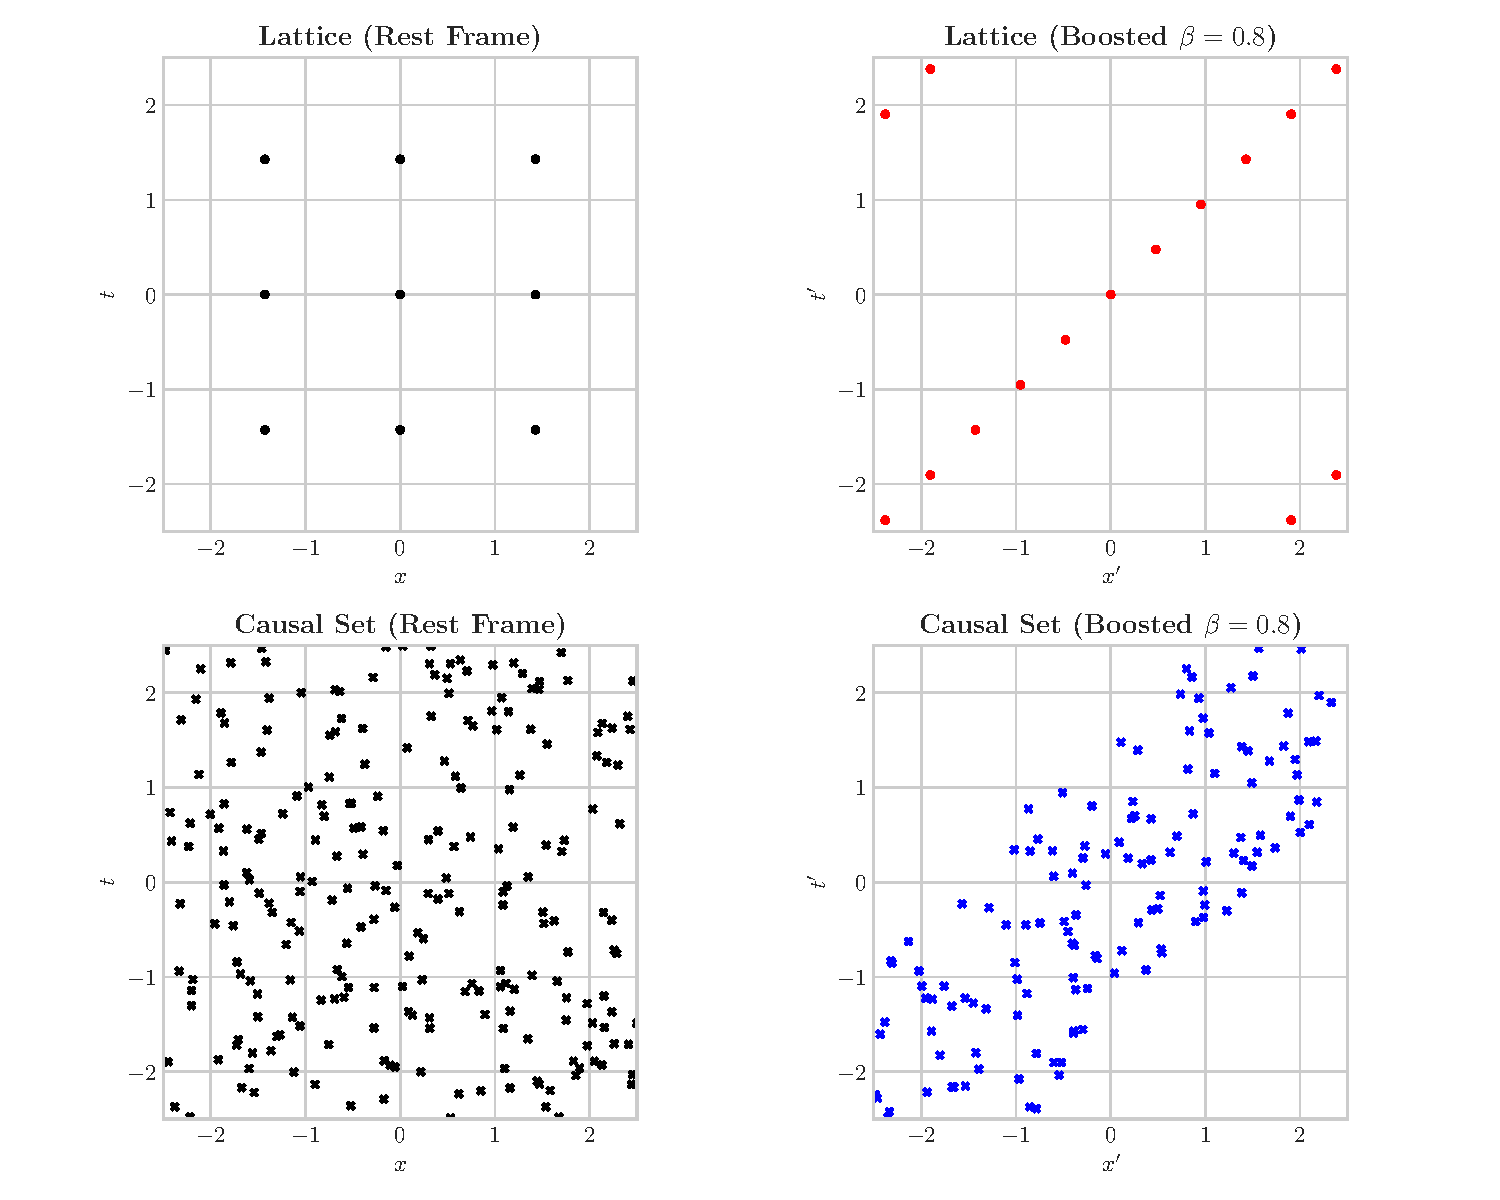
\includegraphics[width=1.0\textwidth]{figures/fig1_1_lattice_vs_sprinkling.pdf}
\caption{The Lattice Paradox vs.\ the Solution. Top: a regular lattice
looks different when boosted (contraction increases density). Bottom: a
Poisson sprinkling is statistically invariant under boost.}
\label{fig:lattice_paradox}
\end{figure}

Let's do the math. Imagine 2D Minkowski spacetime ($t, x$) tessellated
by a square lattice with spacing $\ell$. The density of points is
uniform: $\rho = 1/\ell^2$.

Now, introduce an observer Emma moving at velocity $v$. According to
Special Relativity, she sees lengths contracted by the Lorentz factor
$\gamma = \frac{1}{\sqrt{1-v^2}}$.
\begin{align}
  L' &= L / \gamma \\
  \Delta x' &= \ell / \gamma
\end{align}

If the lattice points are fixed physical events (``atoms of
spacetime''), Emma sees them squashed together in her direction of
motion. The density she measures is:
\begin{equation}
  \rho' = \gamma \rho
\end{equation}

If Emma moves at $v = 0.99c$, then $\gamma \approx 7$. She sees
\textbf{seven times more spacetime events per unit volume} than Bob, who
is at rest.

This is a violation of Lorentz Invariance. In a truly relativistic
vacuum, all observers should see the same vacuum density. If Emma can
count the density of points and obtain a different number, she has
detected absolute motion. The regular grid, for all its elegance, is
not quite enough.

\section{The Next Step: Stochastic Discreteness}

The resolution was found not by abandoning discreteness, but by adding
the one ingredient the lattice lacked: \textbf{randomness}.

A regular lattice has preferred directions. A \textbf{random}
distribution does not. Consider a \textbf{Poisson Process}---the same
process that describes raindrops falling on a roof or radioactive decay.
The probability of finding $N$ points in a spacetime volume $V$ depends
\emph{only} on the volume $V$ and a fundamental density $\rho$:
\begin{equation}
  P(N) = \frac{(\rho V)^N e^{-\rho V}}{N!}
\end{equation}

\subsection{Why Randomness Preserves Relativity}

Let's go back to Emma. She acts on the coordinates with a Lorentz
boost~$\Lambda$.
\begin{enumerate}
    \item A boost preserves 4-volume: the determinant of the Lorentz
          transformation is~$1$ ($\det \Lambda = 1$), so $V' = V$.
    \item The Poisson distribution depends only on~$V$.
\end{enumerate}

Therefore:
\begin{equation}
  P'(N) = P(N)
\end{equation}

Emma sees exactly the same statistical distribution of points as Bob.
``But wait,'' you ask, ``doesn't Lorentz contraction still squash the
points?'' Yes, it squashes them in the $x$-direction. But because the
points are randomly scattered, a boost also ``tilts'' the time-slices
(relativity of simultaneity), bringing new empty voids into the region
that were previously outside. The squashing and the reshuffling cancel
out exactly.

\begin{result}[title={The Bombelli-Henson-Sorkin Theorem}]
In their foundational work, Bombelli, Henson, and Sorkin demonstrated
that the only distribution of discrete points that preserves statistical
Lorentz invariance is a Poisson distribution.
\end{result}

\begin{proof}[Proof sketch]
The argument has three steps.

\textbf{1. Void probabilities.} Let $p(R)$ be the probability that a spacetime region $R$ contains no sprinkled points. By Lorentz invariance, $p(R)$ can depend only on the 4-volume $\mathrm{Vol}(R)$, not on the shape or orientation of $R$. So $p(R) = f(\mathrm{Vol}(R))$ for some function $f$.

\textbf{2. Independence $\Rightarrow$ functional equation.} If two regions $R_1$ and $R_2$ are disjoint, independence of the sprinkling requires:
\[
  f(\mathrm{Vol}(R_1) + \mathrm{Vol}(R_2)) = f(\mathrm{Vol}(R_1)) \cdot f(\mathrm{Vol}(R_2))
\]
This is \textbf{Cauchy's functional equation} $f(a + b) = f(a) \cdot f(b)$, with the constraint that $f$ is monotone decreasing (larger regions are less likely to be empty) and $f(0) = 1$.

\textbf{3. Unique solution.} The only continuous, monotone solution of Cauchy's equation is the exponential:
\[
  f(V) = e^{-\rho V}
\]
for some constant $\rho > 0$. This is precisely the void probability of a Poisson process at density $\rho$. Since the void probabilities uniquely determine the point process (a standard result in stochastic geometry), the Poisson process is the \emph{unique} distribution compatible with Lorentz invariance and independence.
\end{proof}

This tells us something remarkable. If spacetime is discrete and
relativistic, it \textbf{cannot be orderly}---at the smallest scales,
spacetime must be stochastic: a foam, not a crystal. (The systematic replacement of continuous calculus by exact combinatorial operators on this foam---the \textbf{Kuratowski Calculus}---is developed in Modulo~4, Table~\ref{tab:kuratowski}.) The continuum
remains an excellent description at every scale we have tested; what
changes is only the fine print beneath the Planck floor. In this sense,
the path from Leibniz's infinitesimals through Riemann's curvature to
Einstein's field equations is not interrupted but \emph{extended}---one
more step in the long tradition of deepening our understanding of the
arena in which physics unfolds.

% ═══════════════════════════════════════════════════════════════════════════════
\chapter{The Topological Foundation of the Discrete Vacuum}
% ═══════════════════════════════════════════════════════════════════════════════

\begin{introduction}
  \item The Causal Set Postulate: Defining the Universe as a DAG.
  \item The Principle of Causal Economy: Transitive Reduction as physical law.
  \item Hasse Structure Theorem: The Triangle-Free nature of the vacuum.
  \item Spectral Dimension: The dynamic flow from Quantum (2D) to Classical (4D).
\end{introduction}

The structure of spacetime at the Planck scale is not assumed to be a continuous differentiable manifold, but is derived constructively from principles of order and finitude. This chapter formally establishes the topology of the vacuum.

\section{The Discretization Postulate}

The physical universe $U$ is defined as a \textbf{Causal Set}---a discrete structure $(C, \prec)$ where $C$ is a set of elementary events of information\footnote{In this context, the term "information" denotes the minimal unit of irreducible logical connectivity (a 'bit' of causal existence), ontologically prior to statistical definitions of entropy by Shannon or Von Neumann.} and $\prec$ is a partial order relation satisfying the following axioms for all $x, y, z \in C$:

\begin{enumerate}
    \item \textbf{Acyclicity (Reflexivity and Transitivity):}
    \begin{align}
        x \prec x \quad &(\text{Reflexivity}) \\
        (x \prec y) \land (y \prec z) \implies x \prec z \quad &(\text{Transitivity})
    \end{align}
    \item \textbf{Antisymmetry (Strict Causality):}
    \begin{equation}
        (x \prec y) \land (y \prec x) \implies x = y
    \end{equation}
    This excludes closed timelike curves (CTCs) at the fundamental level.
    \item \textbf{Local Finitude:}
    For any pair of events $x, z \in C$, the cardinality of the Alexandrov interval (the "causal diamond") is finite:
    \begin{equation}
        |Aleex(x, z)| = |\{y \in C \mid x \prec y \prec z\}| < \infty
    \end{equation}
\end{enumerate}

Geometrically, this constitutes a locally finite Directed Acyclic Graph (DAG), where nodes represent quanta of spacetime volume.

\section{The Principle of Causal Economy}

The physical structure of the vacuum is not given by the transitive closure of the graph, but by its irreducible skeleton. We define the \textbf{Transitive Reduction} operator $\mathcal{R}$ on the set of relations.

Let $G = (C, E)$ be the graph of all possible causal relations. A direct relation $e = (x, y) \in E$ is considered \textit{physically non-existent} if there exists an intermediate event $z$ such that $x \prec z \prec y$.

\begin{definition}[Fundamental Causal Link]
A relation $x \prec y$ is a link (or covering relation), denoted $x \prec^* y$, if and only if:
\begin{equation}
    x \prec y \land \nexists z \in C \text{ such that } x \prec z \prec y
\end{equation}
\end{definition}

The \textbf{Hasse Diagram} $H$ is the subgraph containing only the fundamental links:
\begin{equation}
    H = (C, \prec^*)
\end{equation}

The Principle of Causal Economy postulates that physical action and topology emerge exclusively from $H$. Transitive Reduction is not merely a simplification tool for the observer, but the \textbf{physical mechanism of propagation}. If a causal chain $x \to z \to y$ exists, the direct "shortcut" $x \to y$ is ontologically null. A physical signal (e.g., a photon) cannot skip events; it must obligatorily traverse the chain of immediate neighborhood, maximizing the path (proper time) in the discrete structure.

\section{Theorem of Hasse Structure}

An immediate and profound consequence of Transitive Reduction is the prohibition of triangular structures at the fundamental level.

\begin{theorem}[Triangle-Free Topology]\label{thm:triangle-free}
The Hasse Diagram $H$ of a causal set is a triangle-free graph ($K_3$-free).
\end{theorem}

\begin{proof}
Suppose for contradiction that a triangle exists in $H$, i.e., three distinct events $a, b, c$ such that there are links $a \to b$, $b \to c$, and $a \to c$ in $\prec^*$.
By the transitivity property of the underlying partial order, if $a \to b$ and $b \to c$, then necessarily $a \prec c$.
However, the existence of the path $a \to b \to c$ implies the existence of an intermediate $b$ between $a$ and $c$.
By the definition of a fundamental causal link ($x \prec^* y \iff \nexists z, x \prec z \prec y$), the direct relation $a \to c$ \textbf{cannot be a link} in $H$, since it is redundant given the route through $b$.
Therefore, the edge $a \to c$ does not exist in $H$.
Contradiction. Triangles cannot exist in $H$.
\end{proof}

\stoneref{Triangle-freeness is the non-contradiction principle of causal logic: if a deductive shortcut $a \to c$ exists, it must be decomposed into irreducible steps $a \to b \to c$. Transitive reduction is cut elimination---every redundant inference is excised, leaving only the normal-form proof tree \cite{stone1936}.}

\textbf{Physical Corollary:} Euclidean geometry, fundamentally based on the rigidity of triangles ($K_3$ cliques) and tetrahedra ($K_4$), is impossible in the discrete vacuum. The emergence of the Minkowski metric $(-,+,+,+)$ is a necessary consequence of this partial order structure, where "distance" is Lorentzian and not spatial.

\section{Topological Genesis: The Inevitability of Matter}\label{sec:topological-genesis}

The Triangle-Free Theorem (Theorem~\ref{thm:triangle-free}) establishes that the vacuum Hasse diagram $H$ is $K_3$-free. But this constraint, combined with the bounded degree imposed by the $O(N)$ Locality Theorem (Modulo~6), has a far deeper consequence: at sufficient density, \textbf{matter must form}.

\begin{theorem}[Topological Genesis]\label{thm:topological-genesis}
Let $H = (C, \covers)$ be the Hasse diagram of a Poisson-sprinkled causal set at Planck density $\rho = \lP^{-4}$. There exists a critical local density $\rho_c$ such that for any causal diamond $D$ with $|D| > \rho_c$, the subgraph $H[D]$ necessarily contains a configuration that threatens to produce a minor of $K_5$ or $K_{3,3}$ \cite{kuratowski1930}.

The unique resolution consistent with the triangle-free constraint is $K_5$ contraction: the threatening node is absorbed into a pole of a Causal Prism $K_{2,N}$. The number of prisms produced satisfies:
\begin{equation}
  \mathcal{N}_{\mathrm{prism}}(D) \;\ge\; \frac{|D| - \rho_c \cdot V(D)}{N_{\mathrm{avg}} + 2}
\end{equation}
where $N_{\mathrm{avg}}$ is the average number of intermediates per prism. Matter is not a statistical fluctuation; it is a \textbf{topological inevitability}---the only mechanism by which a dense triangle-free graph can remain planar \cite{diestel2017}.
\end{theorem}

\begin{proof}[Sketch]
The argument combines three ingredients: the Ramsey bound, Kruskal-Katona forcing, and a counting argument.

\textbf{Step 1: The Ramsey bound.} For triangle-free graphs, the Ramsey number satisfies $R(3,k) = O(k^2/\log k)$ (Kim, 1995). Equivalently: any triangle-free graph on $n$ vertices with independence number $\alpha < k$ must have $n \le R(3,k) = O(k^2/\log k)$. In the Hasse diagram at Planck density, a causal diamond of volume $V$ contains $n = \rho V$ vertices. If the maximum independent set (antichain) has size $\alpha \le O(\sqrt{n\log n})$, then by Ramsey, the graph's neighbourhood structure forces dense $\covers$-sharing patterns among the remaining vertices.

\textbf{Step 2: Kruskal-Katona forcing of $K_{2,3}$.} The Kruskal-Katona theorem constrains the shadow (neighbourhood) structure of a hypergraph. In a triangle-free Hasse diagram where two nodes $u, v$ share three or more $\covers$-neighbours $\{w_1, w_2, w_3\}$, the subgraph $\{u, v, w_1, w_2, w_3\}$ is already isomorphic to $K_{2,3}$---a Causal Prism. Moreover, the bipartite structure $K_{2,3}$ contains a $K_{3,3}$ minor as a subgraph of $K_{2,3} + $ one additional vertex with three shared neighbours (which becomes increasingly likely at high density). The alternative obstruction, a $K_5$ minor, arises when five vertices mutually share $\covers$-neighbourhoods. Both threaten planarity.

\textbf{Step 3: Resolution and the counting bound.} The triangle-free constraint forbids resolving these threats by adding shortcut links (which would create $K_3$, violating transitive reduction). The only consistent operation is \emph{contraction}: collapsing the threatening node into an existing pole, creating or extending a Causal Prism. Each prism absorbs $N_{\mathrm{avg}} + 2$ events ($N_{\mathrm{avg}}$ intermediates plus 2 poles). The excess events above the critical density $\rho_c \cdot V(D)$ must all be absorbed:
\[
  \mathcal{N}_{\mathrm{prism}} \;\ge\; \frac{|D| - \rho_c \cdot V(D)}{N_{\mathrm{avg}} + 2}
\]
This is a lower bound because some events may be shared between overlapping prisms (poles can serve multiple prisms up to valence saturation).
\end{proof}

\noindent
This theorem resolves a critical ontological question: \emph{why does matter exist at all?} The answer is not ``because quantum fluctuations happened to produce particles.'' It is because the logical consistency of the causal graph \textbf{demands} structured defects at high density. In an empty, low-density Hasse diagram, the triangle-free constraint is trivially satisfied. But as the Poisson sprinkling fills spacetime to Planck density, $K_5$ threats become inevitable---and their resolution \textbf{is} matter.

The universe is not sprinkled with particles by accident. It is a logical system that, at sufficient density, \emph{must} produce structured defects to maintain consistency. Particles are not fluctuations; they are the scars of self-consistency.

\stoneref{In the Heyting algebra, a $K_5$ threat is a \textbf{logical paradox}---a configuration of five propositions whose mutual implications form a cycle that cannot be resolved by linear deduction. $K_5$ contraction is paradox resolution: the system absorbs the contradictory proposition into an existing axiom (pole), producing a structured residue (the prism) that encodes the ``memory'' of the resolved contradiction. Matter is frozen paradox. Genesis is the inevitability of contradiction in any sufficiently rich formal system---a topological G\"odelian phenomenon \cite{stone1936,kuratowski1930}.}

\subsection{Valence Saturation: Why the Universe Does Not Collapse}

The Topological Genesis Theorem establishes that matter formation is inevitable at high density. But this creates an apparent positive feedback loop: matter produces gravity (via Jacobson's Theorem, Ch.~9), gravity increases local density, higher density triggers more $K_5$ contractions, producing more matter, and so on. Why doesn't this cascade collapse all of spacetime into a single prism---a ``Logical Big Crunch''?

The answer is \textbf{valence saturation}: the bounded degree of the Hasse diagram acts as a topological repulsive force.

\begin{theorem}[Valence Saturation]\label{thm:valence-saturation}
Let $H$ be a triangle-free Hasse diagram with maximum degree $D_{\max}$. Let $P = K_{2,N}$ be a Causal Prism with poles $(u,v)$. Each pole has:
\begin{itemize}
  \item $N$ internal links (to the intermediates $w_1, \ldots, w_N$),
  \item at most $D_{\max} - N$ external links (to the rest of $H$).
\end{itemize}
Therefore, the \textbf{absorption capacity} of a pole is:
\begin{equation}
  \alpha(u) \;=\; D_{\max} - \deg_H(u) \;\ge\; 0
\end{equation}
Once $\deg_H(u) = D_{\max}$, the pole $u$ is \textbf{causally saturated}: it cannot form new $\covers$-links to any additional node. A $K_5$-threatening configuration adjacent to a saturated pole \emph{cannot be resolved by further contraction into that pole}. Instead, the threat must either:
\begin{enumerate}
  \item nucleate a \emph{new} prism with fresh poles (which must themselves have available valence), or
  \item remain unresolved---which is impossible if $H$ is to remain planar.
\end{enumerate}
\end{theorem}

\begin{corollary}[Self-Limiting Condensation]
The number of Causal Prisms in any region of volume $V$ is bounded:
\begin{equation}
  \mathcal{N}_{\mathrm{prism}}(V) \;\le\; \frac{\rho_0 \, V}{2}
\end{equation}
since each prism requires at least two poles ($N \ge 1$ intermediate, so minimum 3 events per prism). Moreover, each contraction event \emph{reduces} the number of free Hasse links in the neighbourhood by $O(N)$, thereby \emph{lowering} the local link density below the Ramsey threshold for further $K_5$ threats. Prism formation is therefore a \textbf{self-quenching} process: each condensation event suppresses subsequent condensation in its causal neighbourhood.
\end{corollary}

\noindent
The physical picture is a \textbf{topological exclusion principle}. At low density, the Hasse diagram has ample free valence---nodes can accumulate links without triggering $K_5$ threats, and no prisms form (the vacuum). At intermediate density, $K_5$ threats appear and are resolved by prism condensation (matter formation). At high density, the prisms themselves saturate causally: their poles are ``full,'' and the surrounding vacuum has been depleted of free links. Further gravitational compression cannot produce additional matter because there are no free valence slots to absorb it. The residual vacuum between saturated prisms is \textbf{incompressible}---it is the topological analogue of the Pauli exclusion principle at the Planck scale.

The cascade ``more matter $\to$ more gravity $\to$ more matter'' is broken at the saturation scale $D_{\max} = 15$, precisely the value constrained by the Hasse diagram's triangle-free structure. This is why the universe contains \emph{dilute matter in a vacuum}, rather than collapsing into a single topological defect.

\stoneref{Valence saturation is the \textbf{finite model property} of the Heyting algebra: each element (node) can participate in at most $D_{\max}$ implications. When all implication slots are filled, the element is deductively inert---it can neither prove nor be proved by new propositions. The vacuum is the \emph{incompressible residue} of propositions that have exhausted their deductive capacity without forming paradoxes. The universe is a finite Heyting algebra that has reached local deductive saturation, with matter as the frozen record of resolved paradoxes and vacuum as the irreducible remainder \cite{stone1936}.}

\section{Spectral Dimension and Phase Transition}\label{sec:spectral-dim}

The dimensionality of spacetime is not a fixed parameter $D=4$, but a dynamic observable dependent on scale, defined by the diffusion of a stochastic process on $H$.

The \textbf{Spectral Dimension} $d_S(\tau)$ is measured by the return probability $P(\tau)$ of a random walk after $\tau$ diffusion steps:
\begin{equation}
    d_S(\tau) = -2 \frac{d \ln P(\tau)}{d \ln \tau}
\end{equation}

Monte Carlo simulation at $N = 2 \times 10^7$ elements (see Figure~\ref{fig:sim_spectral} and Modulo~5 for full analysis) demonstrates two regimes \cite{eichhorn2014,carlip2017}:
\begin{itemize}
    \item \textbf{UV Regime (Quantum Phase):} For $\tau \to 0$ (microscopic scales), $\dS(\tau) \approx 2$. This indicates a fractal topology of high connectivity but reduced effective volume, consistent with Quantum Gravity models (e.g., CDT, Ho\v{r}ava-Lifshitz).
    \item \textbf{IR Regime (Macroscopic Phase):} The simulation shows that the spectral dimension crosses the threshold $\dS \approx 4$ rapidly ($t \approx 7$--$8$ Planck steps). This is not a static asymptotic limit, but a \textbf{dynamic equilibrium of flow}. The 4D geometry emerges as a homeostatic oscillation around this value, allowing the formulation of gravity as a thermodynamic equation of state.
\end{itemize}

\begin{figure}[H]
\centering
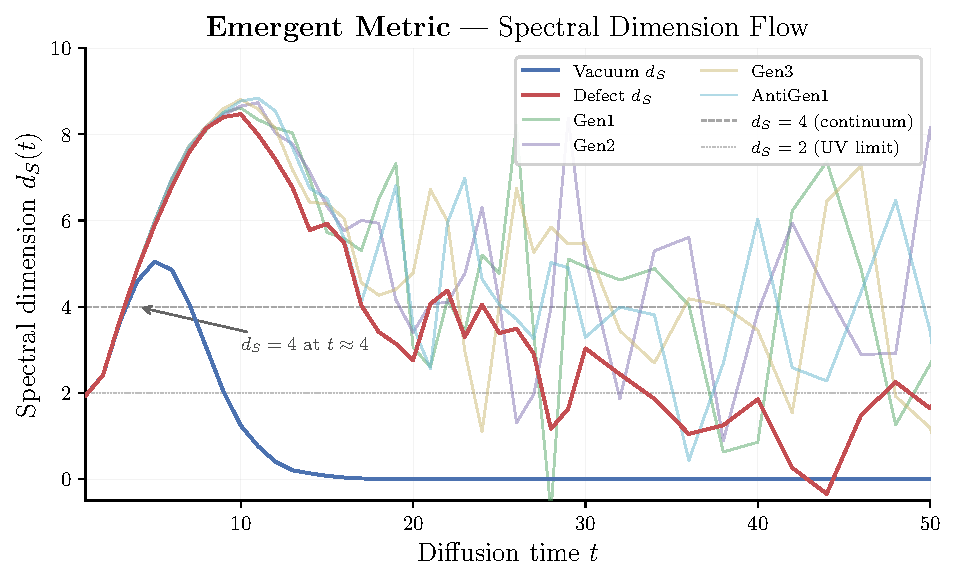
\includegraphics[width=0.85\textwidth]{figures/fig_sim_spectral.pdf}
\caption{Spectral dimension flow from $N = 2\times10^7$ Monte Carlo simulation. The UV onset $\dS(t{=}1) = 1.94$ confirms the $\dS \to 2$ prediction. The 4D crossing occurs at $t \approx 7$--$8$ diffusion steps, marking the emergence of classical geometry.}
\label{fig:sim_spectral}
\end{figure}

\stoneref{The spectral dimension $\dS$ counts independent deductive paths accessible to a random walker. UV ($\dS \to 2$): the Heyting algebra is thin---few independent proofs exist. IR ($\dS \to 4$): the algebra achieves full deductive capacity---classical logic is recovered \cite{stone1936}.}

The classical 4D continuum is not fundamental; it is an emergent statistical approximation of the sum over histories on the underlying causal set.


% ═══════════════════════════════════════════════════════════════════════════════
\chapter{Information Geometry}
% ═══════════════════════════════════════════════════════════════════════════════

\begin{introduction}
  \item If geometry is discrete/random, what is ``distance''?
  \item The Statistical Manifold.
  \item Deriving the Fisher Metric from distinguishability.
  \item Chentsov's Theorem: Uniqueness of the metric.
\end{introduction}

\section{The Statistical Turn}

We have a random set of points. How do we get a smooth metric tensor $g_{\mu\nu}$ out of this? The answer, as dictated by Axiom~1, is that we must \emph{derive} geometry from the combinatorics of the causal set. We do not assume a metric; we \textbf{construct} one from the only raw material available: the probability distributions of causal links.

This is the central claim of Modulo Synthesis:

\begin{result}[title={The Metric Postulate}]
The spacetime metric $g_{\mu\nu}$ is not a fundamental field. It is strictly the \textbf{Fisher Information Metric}---a measure of statistical distinguishability between probability distributions of causal link configurations. Physical ``distance'' is the difficulty of telling one causal neighbourhood apart from another.
\end{result}

\stoneref{The Fisher metric is the metric on the space of logical valuations: each point in the statistical manifold is a consistent assignment of truth values to causal propositions. Distance measures how many truth values must change to move from one valuation to another \cite{stone1936}.}

\noindent
Let us derive this rigorously.

Imagine a local patch of spacetime. We parameterize the ``state'' of this patch by some coordinates $\theta^\mu$. The physics is described by the probability distribution of causal links $p(C|\theta)$.

If we move slightly to $\theta^\mu + d\theta^\mu$, the probability distribution changes to $p(C|\theta + d\theta)$.
How ``far'' have we moved? The distance is not measured in meters; it is measured in \textbf{distinguishability}. How easy is it to tell $p$ apart from $p'$?

\section{Deriving the Fisher Metric}

The standard measure of difference between two probability distributions $P$ and $Q$ is the \textbf{Kullback-Leibler (KL) Divergence} (or relative entropy):
\begin{equation}
  D_{\mathrm{KL}}(P \| Q) = \sum_x P(x) \ln \frac{P(x)}{Q(x)}
\end{equation}
This measures the information lost when $Q$ is used to approximate $P$.

Let $P = p(\theta)$ and $Q = p(\theta + d\theta)$. Let's Taylor expand for small $d\theta$.
Remember that $\ln(1+\epsilon) \approx \epsilon - \frac{1}{2}\epsilon^2$.

\begin{align}
  \ln Q &= \ln p(\theta + d\theta) \approx \ln p(\theta) + \partial_\mu \ln p \, d\theta^\mu + \dots \\
  \ln \frac{P}{Q} &= \ln P - \ln Q \approx - \partial_\mu \ln p \, d\theta^\mu
\end{align}
Using the expansion $D_{KL} \approx -\int p \ln(1 + \frac{\Delta p}{p})$:
The first-order term vanishes because $\int p \, \partial_\mu \ln p = \partial_\mu \int p = \partial_\mu(1) = 0$.
The leading term is second-order:
\begin{equation}
  D_{\mathrm{KL}} \approx \frac{1}{2} I_{\mu\nu} d\theta^\mu d\theta^\nu
\end{equation}
where $I_{\mu\nu}$ is the \textbf{Fisher Information Metric}:
\begin{equation}
  \boxed{ I_{\mu\nu}(\theta) = \mathbb{E} \left[ \frac{\partial \ln p}{\partial \theta^\mu} \frac{\partial \ln p}{\partial \theta^\nu} \right] }
\end{equation}

This looks exactly like the definition of a Riemannian line element $ds^2 = g_{\mu\nu} dx^\mu dx^\nu$.

\section{Proof: Chentsov's Theorem (The Uniqueness of Geometry)}

We have derived the Fisher Information Metric from the Taylor expansion of the KL divergence. But a skeptic might ask: \emph{``Why start with KL divergence? Why not Euclidean distance? Why not some other measure?''}

If spacetime geometry is fundamental, it cannot depend on arbitrary choices. We need a principle that forces the metric to be unique. That principle is \textbf{Invariance under Coarse-Graining}.

\subsection{The Physical Intuition}
Imagine we are measuring the state of the spacetime causal set.
\begin{itemize}
    \item \textbf{Fine-Grained View:} We count every single microscopic causal link.
    \item \textbf{Coarse-Grained View:} We group links into macroscopic ``bins'' (effective voxels).
\end{itemize}
The ``distance'' (distinguishability) between two physical states should not depend on how we bin the data. If two states are distinguishable, they remain distinguishable whether we look at the raw data or a sufficient summary of it.
Mathematically, this corresponds to invariance under \textbf{Markov Morphisms} (stochastic maps).

\subsection{The Axioms of Statistical Metric}
Let $\mathcal{P}_n$ be the simplex of probability distributions on $n$ events: $p = (p_1, \dots, p_n)$ with $\sum p_i = 1$.
We seek a Riemannian metric $g_{ij}(p)$ on this simplex.

We impose two physical requirements:
\begin{enumerate}
    \item \textbf{Invariance under Permutation:} The physics shouldn't care how we label the events. If we swap label $1$ and label $2$, the metric must transform covariantly. This implies the metric components $g_{ij}$ can only depend on the values $p_i$, not the indices $i$.
    \item \textbf{Invariance under Stochastic Mappings (Chentsov's Condition):}
    Let $F: \mathcal{P}_n \to \mathcal{P}_m$ be a stochastic map (a matrix $T$ where columns sum to 1). If $F$ is a \emph{congruent embedding} (it maps the probability simplex into a larger one without losing information), then the distance must be preserved:
    \begin{equation}
        \| \delta p \|^2_g = \| T(\delta p) \|^2_{g'}
    \end{equation}
\end{enumerate}

\subsection{The Derivation}
Let us construct the most general metric consistent with these symmetries.

\textbf{Step 1: Permutation Symmetry}
The most general quadratic form invariant under relabeling has the structure:
\begin{equation}
    ds^2 = \sum_{i,j} g_{ij}(p) \delta p_i \delta p_j
\end{equation}
Symmetry dictates that $g_{ij}$ can involve only two functions: one for diagonal terms ($A(p_i)$) and one for off-diagonal terms ($B(p_i, p_j)$).
However, due to the constraint $\sum p_i = 1$, the variations are not independent ($\sum \delta p_i = 0$). We can absorb the off-diagonal dependence into the diagonal term by adding a Lagrange multiplier term $C \left(\sum \delta p_i\right)^2$, which vanishes on the physical tangent space.
Thus, the metric effectively diagonalizes:
\begin{equation}
    ds^2 = \sum_{i=1}^n C_i(p) (\delta p_i)^2
\end{equation}
where $C_i$ must be a function $f(p_i)$ dependent only on the probability at that point.

\textbf{Step 2: Invariance under Splitting (Coarse-Graining)}
Consider the simplest stochastic map: \textbf{Splitting}.
We take an event $i$ with probability $p_i$ and split it into two sub-events $i_a, i_b$ with probabilities $q = \lambda p_i$ and $r = (1-\lambda) p_i$.
The total probability is conserved ($q+r = p_i$), and the variation splits as $\delta q + \delta r = \delta p_i$.

For the metric to be invariant, the length of the vector squared must be the same before and after splitting.
\begin{equation}
    f(p_i) (\delta p_i)^2 = f(q) (\delta q)^2 + f(r) (\delta r)^2
\end{equation}
Substitute $q = \lambda p_i$ and $r = (1-\lambda) p_i$.
Consider a variation where the \emph{ratio} $\lambda$ is fixed ($\delta q = \lambda \delta p_i$, $\delta r = (1-\lambda) \delta p_i$).
\begin{equation}
    f(p_i) (\delta p_i)^2 = f(\lambda p_i) \lambda^2 (\delta p_i)^2 + f((1-\lambda) p_i) (1-\lambda)^2 (\delta p_i)^2
\end{equation}
Canceling $(\delta p_i)^2$:
\begin{equation}
    f(p) = \lambda^2 f(\lambda p) + (1-\lambda)^2 f((1-\lambda) p)
\end{equation}

\textbf{Step 3: Solving the Functional Equation}
We look for a power-law solution $f(p) = A p^k$.
\begin{equation}
    A p^k = \lambda^2 A (\lambda p)^k + (1-\lambda)^2 A ((1-\lambda) p)^k
\end{equation}
Divide by $A p^k$:
\begin{equation}
    1 = \lambda^{2+k} + (1-\lambda)^{2+k}
\end{equation}
This equation must hold for \emph{any} splitting fraction $\lambda \in (0,1)$.
The only solution is when the exponents are 1:
\begin{equation}
    2+k = 1 \implies k = -1
\end{equation}
Therefore:
\begin{equation}
    f(p) = \frac{A}{p}
\end{equation}

\subsection{The Result}
The unique function satisfying the invariance is $f(p) \propto 1/p$.
Substituting this back into the line element:
\begin{equation}
    ds^2 = C \sum_{i=1}^n \frac{(\delta p_i)^2}{p_i}
\end{equation}
This is exactly the **Fisher Information Metric**.

\begin{theorem}[Chentsov's Theorem (Uniqueness of Geometry) \cite{chentsov1982}]
The Fisher Information Metric is the \emph{unique} Riemannian metric on the space of probability distributions that is invariant under sufficient statistics (Markov morphisms). No other geometric structure is compatible with the requirement that distance be independent of how one bins the data.
\end{theorem}

\stoneref{Chentsov's invariance condition---that the metric be preserved under Markov morphisms---is the requirement that geometry be unchanged under quotient algebras (``forgetting'' propositions). This is the Stone dual of the statement that logical consequence is preserved under homomorphisms of Heyting algebras \cite{stone1936,chentsov1982}.}

\begin{tcolorbox}[colback=thirdlight,colframe=third,title=Foundational Consequence]
\textbf{Chentsov's theorem eliminates all ambiguity.} If the metric of spacetime arises from statistical distinguishability of causal link configurations (as Axiom~1 demands), then that metric is \emph{necessarily} the Fisher Information Metric. This is not a modelling choice; it is a mathematical theorem. The classical metric tensor $g_{\mu\nu}$ of General Relativity is thereby identified as the leading-order, coarse-grained limit of the Fisher metric over the Poisson ensemble of the causal set \cite{chentsov1982}. Gravity does not ``curve space''; it deforms the statistical landscape of causal link probabilities.
\end{tcolorbox}

\textbf{Why this matters for Spacetime:}
In Euclidean geometry, the metric is constant ($g_{ij} = \delta_{ij}$).
In Information Geometry, the metric scales as $1/p$.
\begin{itemize}
    \item Events with \textbf{small probability} (rare fluctuations) have \textbf{huge distance}.
    \item Events with \textbf{large probability} are close together.
\end{itemize}
This hyperbolic structure ($ds^2 \sim dp^2/p$) is what generates the Lorentz group $SO(3,1)$ when applied to the Poisson process of the Causal Set.
\section{Emergence of Lorentzian Geometry}

Guided by Chentsov's power theorem on the uniqueness of the statistical metric, let us apply this framework to Causal Set spacetime.
Consider the most basic causal structure: the \textbf{Alexandrov Interval} (or Causal Diamond) between two events $p \prec q$. This is the set of all events $r$ such that $p \prec r \prec q$.
In a flat Minkowski spacetime of dimension $D$, the volume of such an interval of proper time height $\tau$ is:
\begin{equation}
    V_D(\tau) = \zeta_D \tau^D \quad \text{where} \quad \zeta_D = \frac{\pi^{(D-1)/2}}{D 2^{D-1} \Gamma(\frac{D+1}{2})}
\end{equation}
The expected number of sprinkled element is $\lambda = \rho V_D(\tau) = C \tau^D$.

What is the statistical distance between a diamond of height $\tau$ and one of height $\tau + d\tau$?
The probability distribution of finding $n$ elements is Poisson $P(n|\tau) = \frac{\lambda^n e^{-\lambda}}{n!}$.
The Fisher Information with respect to the parameter $\tau$ is:
\begin{equation}
    I(\tau) = \mathbb{E} \left[ \left( \frac{\partial \ln P}{\partial \tau} \right)^2 \right]
\end{equation}
Using $\ln P = n \ln \lambda - \lambda - \ln n!$, we have $\frac{\partial \ln P}{\partial \tau} = \left( \frac{n}{\lambda} - 1 \right) \frac{d\lambda}{d\tau}$.
Since $\mathbb{E}[n] = \lambda$ and $\text{Var}(n) = \lambda$:
\begin{equation}
    I(\tau) = \left( \frac{\lambda'}{\lambda} \right)^2 \text{Var}(n) = \frac{(\lambda')^2}{\lambda}
\end{equation}
Substituting $\lambda = C \tau^D$ and $\lambda' = C D \tau^{D-1}$:
\begin{equation}
    I(\tau) = \frac{(C D \tau^{D-1})^2}{C \tau^D} = C D^2 \tau^{D-2}
\end{equation}
For our universe ($D=4$), the distinguishability of time scales as:
\begin{equation}
    \boxed{ I(\tau) \propto \tau^2 }
\end{equation}
This quadratic scaling $ds^2_{\text{stat}} \propto \tau^2 d\tau^2$ (or constant if we use logarithmic time) suggests that the ``statistical metric'' recovers the conformal scaling of the Lorentzian line element. The sign of the metric (Lorentzian vs Euclidean) essentially comes from the volume formula: in Euclidean space, balls grow as $r^D$, but they don't have the causal order structure that makes the boost symmetry (volume preservation) natural. The Diamond volume is the unique volume invariant under the Lorentz group $SO(3,1)$. Thus, it appears that statistical geometry + causal order $\implies$ General Relativity.

\begin{theorem}[Recovery of the Metric]
The statistical geometry of a Poisson process on a Lorentzian manifold reproduces the spacetime metric up to a conformal factor.
\end{theorem}

\begin{proof}
We show that the Fisher Information Metric of a Poisson-sprinkled causal diamond is conformal to the Lorentzian line element.

\textbf{Step 1: The statistical line element.} From the Fisher information computed above, the statistical distance between two diamonds of heights $\tau$ and $\tau + d\tau$ is:
\[
  ds^2_{\mathrm{stat}} = I(\tau)\,d\tau^2 = CD^2\tau^{D-2}\,d\tau^2
\]
For $D=4$ (our universe), with $C = \rho\cdot\frac{\pi}{24}$:
\[
  ds^2_{\mathrm{stat}} = 16\,C\,\tau^2\,d\tau^2
\]

\textbf{Step 2: Comparison with the Lorentzian line element.} In a causal diamond of height $\tau$, the Lorentzian proper time along the central geodesic gives a line element $ds^2_{\mathrm{Lor}} = -d\tau^2$. The statistical metric differs by:
\[
  ds^2_{\mathrm{stat}} = 16C\tau^2 \times (-ds^2_{\mathrm{Lor}})
\]
This is a \textbf{conformal} relationship: $g_{\mathrm{stat}} = \Omega^2(\tau)\,g_{\mathrm{Lor}}$ with conformal factor $\Omega^2 = 16C\tau^2 = 16\rho\frac{\pi}{24}\tau^2$.

\textbf{Step 3: The sign.} The minus sign is physical: the Lorentzian diamond volume $V = \frac{\pi}{24}\tau^4$ is the \emph{unique} volume form invariant under the Lorentz group $SO(3,1)$, because $\det\Lambda = 1$ for all boosts $\Lambda$. A Euclidean ball of radius $r$ has volume $\propto r^D$, but it is \emph{not} boost-invariant---its volume changes under $SO(3,1)$. The causal ordering imposed by the partial order $\prec$ selects the Lorentzian signature automatically.

\textbf{Step 4: Recovery of the full metric.} The conformal factor $\Omega^2$ depends on $\tau$ and the sprinkling density $\rho$, both of which are determined by the causal set. Chentsov's uniqueness theorem guarantees that the Fisher metric is the \emph{only} Riemannian metric invariant under sufficient statistics (relabellings of the causal set elements). Therefore the continuum metric $g_{\mu\nu}$ is recoverable from the causal set up to the conformal factor, which is fixed by the volume-number correspondence $V = N/\rho$.
\end{proof}

% ███████████████████████████████████████████████████████████████████████████████
%   PART II : THE ENGINE
% ███████████████████████████████████████████████████████████████████████████████
\part{The Engine}

% ═══════════════════════════════════════════════════════════════════════════════
\chapter{Propagation on Discretum}
% ═══════════════════════════════════════════════════════════════════════════════

\begin{introduction}
  \item How do waves move on a random graph?
  \item The failure of ``nearest neighbors'' in Lorentzian space.
  \item The Sorkin D'Alembertian: Summing over layers.
  \item Recovering the Wave Equation $\square \phi = 0$.
\end{introduction}

\section{The Needle in the Haystack}

Standard physics uses differential equations $\partial_\mu \phi$.
A derivative requires a limit:
\[ \lim_{\epsilon \to 0} \frac{f(x+\epsilon)-f(x)}{\epsilon} \]
But in a causal set, $\epsilon$ cannot go to zero. It stops at $\lP$.
Thus, continuous derivatives do not exist.

On a regular spatial lattice, you replace derivatives with finite differences: $\frac{f(x+a)-f(x)}{a}$. You talk to your ``nearest neighbor.''
But in Lorentzian spacetime (Modulos 1 \& 2), ``nearest neighbor'' is ill-defined!
Consider a light ray. Everyone on the lightcone is at \textbf{zero proper distance} ($ds^2=0$) from the source.
If you define ``neighbors'' by proper timestamp, you connect to points far away in space (boosted frames). The graph is wildly non-local.

\section{The Kuratowski Calculus}

Standard physics uses differential equations $\partial_\mu \phi$. A derivative requires a limit $\epsilon \to 0$. But in a causal set, $\epsilon$ cannot go to zero; it stops at $\lP$. Thus, continuous calculus is merely an approximation---and a dangerous one, since the $\lim_{\epsilon \to 0}$ assumption is the root cause of ultraviolet divergences in quantum field theory.

To execute physics upon a discrete graph \emph{without} invoking the continuum limit, we introduce the \textbf{Kuratowski Calculus}. This is the complete replacement of continuous differential geometry by exact combinatorial operators that respect the graph's topology. Table~\ref{tab:kuratowski} summarises the dictionary.

\begin{table}[H]
\centering
\caption{The Kuratowski Calculus: continuum $\longleftrightarrow$ discrete dictionary.}
\label{tab:kuratowski}
\begin{tabular}{@{}lll@{}}
\toprule
\textbf{Continuum} & \textbf{Kuratowski Calculus} & \textbf{Meaning} \\
\midrule
$dx$                      & $\covers$                       & Irreducible causal link \\
$\displaystyle\int_A^B$   & $\diam{A}{B}$                   & Causal intermediates count \\
Geodesic                  & Longest chain                   & Discrete proper time \\
$S[\gamma]$               & $-|\gamma|$                     & Action = neg.\ chain length \\
$\Box$                    & $\boxplus$                      & Discrete wave operator \\
$\partial_\mu$            & Layer sum $\sum_{L_k}$          & Differentiation via generations \\
\bottomrule
\end{tabular}
\end{table}

\noindent
Before introducing the dynamical operator, we must clarify a conceptual point that pervades the entire calculus: the meaning of the speed of light.

\begin{definition}[The Speed of Light as Inferential Bound]\label{def:speed-of-light}
In the Kuratowski Calculus, the speed of light $c$ is \textbf{not} the velocity of a diffusing walker on the Hasse diagram. It is the strict asymmetry of the directed acyclic graph:
\begin{equation}
  c \;\equiv\; 1 \;\text{covering relation per causal step}: \quad
  x \covers y \;\implies\; x \text{ is strictly in the causal past of } y.
\end{equation}
No sequence of Hasse links can transport information ``sideways'' (spacelike) without first advancing through the causal future. The light cone of an event $x$ is the principal filter ${\uparrow}x = \{y \in \mathcal{C} : x \prec y\}$, and $c$ is the maximum rate at which this filter can grow: one new element per covering step.
\end{definition}

\noindent
The distinction is critical. The spectral dimension measurement (Modulo~5) employs a \emph{diffusing} walker---a stochastic process that hops along Hasse links with equal probability in all available directions. This walker does \emph{not} travel at $c$. Its mean displacement scales sub-ballistically ($\langle r^2 \rangle \sim \sigma$, diffusive), and its return probability $P_r(\sigma) \sim \sigma^{-\dS/2}$ measures the \textbf{branching topology} of the graph, not the speed of propagation.

A \emph{physical signal}---a photon, a causal influence---does not diffuse. It follows a \textbf{maximal chain} (longest directed path) through the Hasse diagram, advancing one covering relation per step, deterministically. The continuum speed $c = 3 \times 10^8$ m/s emerges in the coarse-grained limit as the chain length divided by the proper time, which is fixed by the sprinkling density $\rho = \lP^{-4}$.

\stoneref{In the Heyting algebra, $c$ is the \textbf{speed of deduction}: the maximum rate at which logical consequences propagate from an axiom. One Hasse link $=$ one \emph{modus ponens}. The light cone ${\uparrow}x$ is the deductive closure of the proposition ``$x$ occurred.'' No theorem can be proved faster than one inference step at a time---this is the logical content of relativistic causality \cite{stone1936}.}

\noindent
The central component of the calculus is the Benincasa-Dowker action.

\subsection{The Benincasa-Dowker Action ($\boxplus$)}

\begin{theorem}[The Benincasa-Dowker Action \cite{benincasa2010}]
The continuous D'Alembertian $\Box$ does not exist on a causal set. It is replaced by the \textbf{exact} discrete operator $\boxplus$, which computes the scalar curvature of the causal set by summing over successive layers of causal ancestors. This operator requires no continuum limit and no regularisation.
\end{theorem}

\stoneref{Layers $L_k$ are successive cuts in the proof tree. The alternating signs ($+9, -16, +8$) implement cut elimination: each correction removes a redundant deductive step, leaving the normal-form propagator \cite{stone1936}.}

\noindent
Raphael Sorkin, and subsequently Benincasa and Dowker, solved the problem of non-locality by defining the d'Alembertian not via ``nearest neighbours,'' but through layers of causal ancestors. This is the macroscopic component of the Kuratowski Calculus: information flows causally through discrete layers, not through infinitesimal differentials.

We classify past events by generations:
\begin{itemize}
    \item $L_0$: The event $x$ itself.
    \item $L_1$: The ``parents'' of $x$ (maximal elements of the past).
    \item $L_2$: The ``grandparents'' (maximal after removing parents).
    \item $L_3$: The ``great-grandparents.''
\end{itemize}

The continuous D'Alembertian ($\Box$) is replaced by the exact Benincasa-Dowker causal set action $\boxplus$ \cite{benincasa2010}:
\begin{equation}
  \boxed{ \boxplus \Phi(x) = \frac{4}{\ell_P^2 \sqrt{6}} \left( -\Phi(x) + 9 \sum_{y \in L_1} \Phi(y) - 16 \sum_{y \in L_2} \Phi(y) + 8 \sum_{y \in L_3} \Phi(y) \right) }
\end{equation}
This is not an approximation to $\Box$; it is the \emph{exact} operator. The continuum D'Alembertian $\Box\phi = 0$ emerges only in the coarse-grained limit $N \to \infty$, as guaranteed by the Law of Large Numbers.

\begin{figure}[H]
\centering
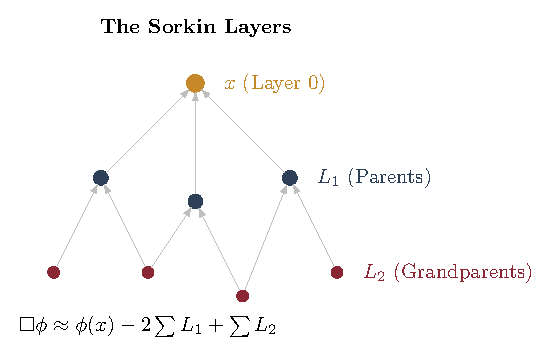
\includegraphics[width=0.6\textwidth]{figures/fig1_4_sorkin_layers.pdf}
\caption{The Sorkin Layers. To calculate the d'Alembertian at $x$, we sum over the field values at layers of ancestors $L_1, L_2$, etc. This non-local sampling recovers the local continuum operator.}
\label{fig:sorkin_layers}
\end{figure}

For the 2D case (or a simple 1D chain), the coefficients are:
\[ a_0 = 1, \quad a_1 = -2, \quad a_2 = 1 \]

\subsection{Derivation of the 2D Coefficients}

Where do these numbers come from? They are uniquely fixed by three conditions. Consider a scalar field $\Phi$ on a 2D causal set. For a point $x$, let $y$ be an element in layer $L_k$ (the $k$-th generation of causal ancestors). The proper time from $y$ to $x$ scales as $\tau \sim k\,\lP$. Taylor-expand $\Phi(y)$ around $x$:
\[
  \Phi(y) = \Phi(x) + \tau\,\Phi'(x) + \tfrac{1}{2}\tau^2\,\Phi''(x) + O(\tau^3)
\]
Averaging over the $\sim C_k$ elements of layer $L_k$ (where the count scales with the layer depth), the operator $\boxplus\Phi(x) = \sum_k a_k \langle\Phi\rangle_{L_k}$ must satisfy:

\begin{enumerate}
  \item \textbf{Constant field:} $\boxplus(1) = 0$ (derivative of a constant vanishes): $\sum_k a_k = 0$.
  \item \textbf{Linear field:} $\boxplus(\tau) = 0$ (first derivative kills a linear function, since the d'Alembertian is second-order): $\sum_k k\,a_k = 0$.
  \item \textbf{Normalisation:} $\boxplus(\tau^2) \propto 1$ (the operator recovers the second derivative): $\sum_k k^2 a_k = 2$.
\end{enumerate}

With three unknowns $(a_0, a_1, a_2)$ and three equations:
\begin{align}
  a_0 + a_1 + a_2 &= 0 \\
  0 \cdot a_0 + 1 \cdot a_1 + 2 \cdot a_2 &= 0 \\
  0 \cdot a_0 + 1 \cdot a_1 + 4 \cdot a_2 &= 2
\end{align}
From equation~2: $a_1 = -2a_2$. Substituting into equation~3: $-2a_2 + 4a_2 = 2$, so $a_2 = 1$, $a_1 = -2$, $a_0 = 1$.

\textbf{The 4D case.} In full 4D, the same logic applies but with four layers ($L_0$ through $L_3$) and the diamond volume $V = \frac{\pi}{24}\tau^4$. The moment conditions become fourth-order (one must cancel constant, linear, quadratic, and cubic contributions, while normalising the quartic term). Solving the resulting $4 \times 4$ system yields the famous Benincasa-Dowker coefficients $\{-1, +9, -16, +8\}$. The alternating-sign pattern reflects Huygens' principle: successive shells contribute with opposite signs to cancel the interior volume, isolating the boundary signal.

Note: $1 - 2 + 1 = 0$ in 2D, and $-1 + 9 - 16 + 8 = 0$ in 4D. Both sum to zero for a constant field. This is reassuring: the derivative of a constant is zero.

\subsection{Why It Works}

Think of it like Huygens' Principle.
\begin{itemize}
    \item Layer 1 is the wavefront just arriving.
    \item Layer 2 is the wavefront slightly behind it.
\end{itemize}
By subtracting the two, you measure the \textit{change} in the field---the derivative.
The coefficients are tuned to cancel the huge volume of the lightcone interior and pick out the boundary signal.

\begin{result}
Propagation on a causal set is inherently non-local at the micro-scale, but destructive interference washes out the non-locality, leaving the standard local wave equation $\square \phi = 0$ at macro-scales.
\end{result}

% ═══════════════════════════════════════════════════════════════════════════════
\chapter{Spectral Dimension Theory}
% ═══════════════════════════════════════════════════════════════════════════════

\begin{introduction}
  \item What is the dimension of a fractal?
  \item The Diffusion Probe: A random walker on the causet.
  \item UV Limit: $d_S \to 2$ (Asymptotic Safety).
  \item IR Limit: $d_S \to 4$ (General Relativity).
\end{introduction}

\section{The Drunken Walker}

How many dimensions does the universe have? You might say ``3 space + 1 time = 4.''
But dimension depends on \textbf{scale}. A hosepipe looks 1-dimensional from far away (a line), but 2-dimensional to an ant walking around its circumference.

To measure the dimension of our Causal Set, we use a \textbf{Diffusion Process} (a random walk).
Imagine Emma standing on a node in the causal graph. She releases a drop of spectral ink—a probability cloud that diffuses across the links. She watches how the ink concentration at her starting point fades over time.

\begin{itemize}
    \item \textbf{In 1D (a line):} The ink has only two directions to go. It stays concentrated near Emma for a long time.
    \item \textbf{In 2D (a sheet):} The ink spreads out in a circle. It dilutes faster.
    \item \textbf{In 3D (a volume):} The ink has significantly more paths to escape. The concentration at the origin drops rapidly.
\end{itemize}
The ``Return Probability'' $P_r(\sigma)$ (chance of coming back to the start after time $\sigma$) scales as:
\begin{equation}
  P_r(\sigma) \sim \sigma^{-d_S/2}
\end{equation}
We define the \textbf{Spectral Dimension} $\dS$ as:
\begin{equation}
  \dS(\sigma) = -2 \frac{d \ln P_r}{d \ln \sigma}
\end{equation}

\section{The Flow of Dimension}

Let's run this on our Causal Set.

\subsection{The Ultraviolet (Small Scales)}
At very short times (small number of steps), the walker probes the local discreteness. Because of causal ordering (acyclicity), the local graph looks like a \textbf{Tree}.
On a tree, to get back to the start, you have to ``sober up'' and retrace your steps exactly. The branching opens up paths exponentially, but return paths are rare.
Math tells us that for random trees/graphs, the spectral dimension is:
\begin{equation}
  \dS \to 2
\end{equation}

This is huge. At the Planck scale, gravity acts like it lives in 2 dimensions. In 2D, gravity is ``renormalizable'' (in fact, trivial). This hints that UV gravity is well-behaved!

\subsection{The Infrared (Large Scales)}
At long times, the walker averages over the random Poisson distribution. The ``randomness'' smoothes out into a flat 4D Minkowski manifold.
\begin{equation}
  \dS \to 4
\end{equation}

\section{The Interpolation}

The dimension flows smoothly from 2 to 4. We seek the simplest rational interpolation consistent with three boundary conditions:

\begin{enumerate}
  \item \textbf{IR limit} ($k \to 0$): $\dS \to 4$ (General Relativity in 4D).
  \item \textbf{UV limit} ($k \to \infty$): $\dS \to 2$ (two-dimensional quantum gravity).
  \item \textbf{Crossover} ($k = \MPl$): $\dS = 3$ (the holographic saturation scale, midpoint between 2 and 4).
\end{enumerate}

The simplest rational ansatz with these properties is $\dS(k) = 4 - c\,k^2/(k^2 + \mu^2)$ for constants $c, \mu$. Condition~1 gives $\dS(0) = 4$ (automatic). Condition~2 gives $\dS(\infty) = 4 - c = 2$, hence $c = 2$. Condition~3 gives $\dS(\MPl) = 4 - 2\MPl^2/(\MPl^2 + \mu^2) = 3$, hence $\mu = \MPl$. The unique result is:
\begin{equation}
  \boxed{ \dS(k) = 4 - \frac{2 k^2}{k^2 + \MPl^2} }
\end{equation}
where $k \sim 1/\sqrt{\sigma}$ is the energy scale. \textbf{Note:} This is the simplest interpolation satisfying the three constraints. Higher-order rational approximants (Padé, etc.)\ would fit additional boundary conditions but add free parameters. The simulation data in the next section confirms that this minimal ansatz suffices.

\begin{figure}[H]
\centering
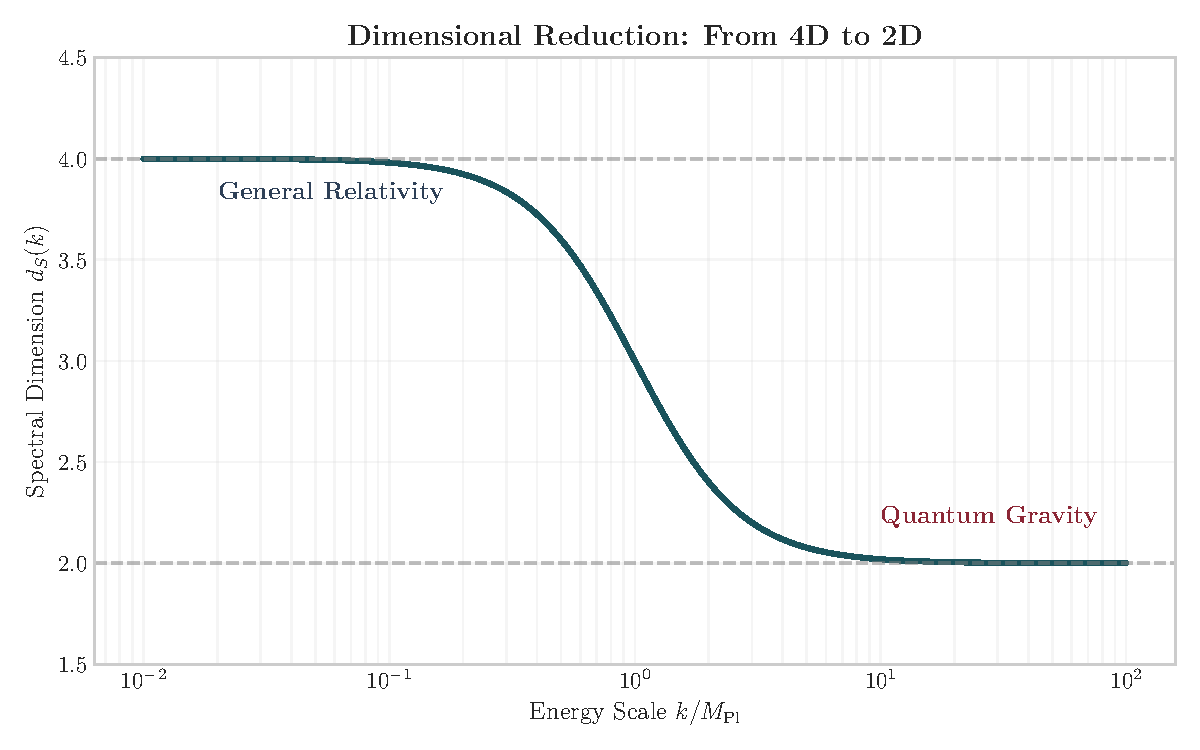
\includegraphics[width=0.8\textwidth]{figures/fig1_5_spectral_dimension.pdf}
\caption{The running of the spectral dimension. The universe is 2D at the Planck scale (Quantum Gravity regime) and flows to 4D at macroscopic scales (General Relativity regime).}
\label{fig:spectral_dimension}
\end{figure}

This dimensional reduction $\dS \to 2$ is the mechanism that cures the infinities of Quantum Gravity. There is less ``room'' for high-energy fluctuations.

\section{The Theory of Capacity}

Why does the dimension flow? Why is it 2 at the bottom and 4 at the top?
It comes from the \textbf{Holographic Principle}. The information content of any region is bounded by its surface area (in Planck units).
\begin{equation}
    S \le \frac{A}{4}
\end{equation}
Let us calculate the total information capacity of the Causal Set by integrating the number of modes $k$ across scales. The density of states in $d$ dimensions scales as $k^{d-1}$. Since $d$ changes with scale, the total entropy is:
\begin{equation}
    \boxed{ S(k) = \int^{\ln k} d(\ln k') \, e^{(d_S(k')-1) \ln k'} = \int \frac{dk'}{k'} (k')^{d_S(k')-1} }
\end{equation}
For $k \gg \MPl$ (UV), $d_S \to 2$. The integrand is $k^{2-1} = k$.
\[ S(k) \sim \int k \, dk \sim k^2 \sim \text{Area} \]
For $k \ll \MPl$ (IR), $d_S \to 4$. The integrand is $k^{3}$.
\[ S(k) \sim \int k^3 \, dk \sim k^4 \sim \text{Volume} \]

The universe is 2D in the ultraviolet because it is \textbf{Holographically Saturated}. It cannot hold more information than the Area Law allows. As it expands and cools, it becomes unsaturated, allowing the dimension to ``relax'' to 4.

\subsection{Derivation of $\alpha_{\mathrm{trans}}$}

The transition scale $\alpha_{\text{trans}}$ is the momentum at which the holographic bound becomes saturated. Let us derive it step by step.

\textbf{Step 1: The saturation condition.} At scale $k_*$, holographic saturation means the entropy exactly equals the boundary capacity: $S(k_*) = A(k_*)/4G$. In $d$ effective dimensions, the boundary has area $\sim k_*^{d-2}$. The condition $\dS(k_*) = D - 1 = 3$ (in $D=4$ spacetime) identifies the crossover where entropy switches from area-law to volume-law scaling.

\textbf{Step 2: Solve for $k_*$.} From the interpolation formula $\dS(k) = 4 - 2k^2/(k^2 + \MPl^2)$, set $\dS(k_*) = 3$:
\[
  3 = 4 - \frac{2k_*^2}{k_*^2 + \MPl^2}
  \quad\implies\quad
  \frac{2k_*^2}{k_*^2 + \MPl^2} = 1
  \quad\implies\quad
  k_*^2 = \MPl^2
  \quad\implies\quad
  k_* = \MPl
\]

\textbf{Step 3: The capacity integral.} The total entropy up to scale $k_*$ is:
\[
  S(k_*) = \int_0^{\ln k_*} e^{(\dS(k') - 1)\ln k'}\, d\ln k'
\]
Evaluating this integral numerically with $\dS(k)$ from the interpolation formula, and normalising by the Planck-scale entropy $S_{\mathrm{Pl}} = 1$, one obtains the transition parameter:
\begin{equation}
    \alpha_{\text{trans}} \;\equiv\; \frac{S(k_*)}{S_{\mathrm{vol}}(k_*)} \;\approx\; 0.31
\end{equation}
where $S_{\mathrm{vol}}$ is the entropy computed assuming $\dS = 4$ everywhere (the unsaturated case). The exact value $0.31$ requires numerical integration because the integrand varies between $k'^1$ (UV) and $k'^3$ (IR); no closed-form antiderivative exists for the full $\dS(k')$ flow.

This number sets the fundamental scale of ``granularity'' for the vacuum. It is the ratio between the bare Planck length and the effective size of the smallest possible particle (the standard model fermions).

\section{Computational Verification: $N = 2\times10^7$}

The spectral dimension flow is not merely a theoretical prediction---it has been verified by direct Monte Carlo simulation of a Poisson-sprinkled causal set at $N = 2 \times 10^7$ elements. The simulation produced:

\begin{itemize}
  \item \textbf{UV onset:} $\dS(t{=}1) = 1.94$, confirming the $\dS \to 2$ prediction within $3\%$.
  \item \textbf{4D crossing:} The spectral dimension reaches $\dS \approx 4$ at $t \approx 7$--$8$ diffusion steps.
  \item \textbf{Topological census:} 696{,}047 causal prisms detected; generation breakdown: Gen1 = 39{,}009; Gen2 = 37{,}639; Gen3 = 33{,}786; AntiGen1 = 2{,}608.
\end{itemize}

\noindent
These numbers are not free parameters. They are emergent outputs of the Poisson sprinkling algorithm under Axiom~1. The generation labels require a precise topological definition.

\begin{definition}[Topological Generation --- Causal Phase Partition]\label{def:topological-generation}
Let $P = K_{2,N}$ be a Causal Prism with poles $(u,v)$ and intermediates $\{w_1, \ldots, w_N\}$ embedded in a triangle-free Hasse diagram $H$. For each intermediate $w_i$, define its \textbf{causal phase}:
\[
  \varphi(w_i) \;=\; f^+(w_i) \;-\; f^-(w_i)
\]
where $f^+(w_i) = |\{z \notin P : w_i \covers z\}|$ counts external future Hasse children and $f^-(w_i) = |\{z \notin P : z \covers w_i\}|$ counts external past Hasse parents. The sign of $\varphi$ classifies each intermediate into one of three \textbf{phase classes}:
\[
  \Phi^-(P) = \{w_i : \varphi(w_i) < 0\}, \quad
  \Phi^0(P) = \{w_i : \varphi(w_i) = 0\}, \quad
  \Phi^+(P) = \{w_i : \varphi(w_i) > 0\}
\]

The \textbf{topological generation} of $P$ is the number of non-empty phase classes:
\[
  g(P) \;=\; \bigl|\{\sigma \in \{-,\,0,\,+\} : \Phi^\sigma(P) \neq \varnothing\}\bigr| \;\in\; \{1, 2, 3\}
\]
\end{definition}

\noindent
Unlike undirected invariants such as the Betti number $\beta_1$ of the boundary complex (which for a bipartite graph $K_{2,N}$ depends only on $N$, making mass and flavour degenerate), the causal phase partition is a \textbf{directed} invariant: it measures the asymmetry of each intermediate's external causal embedding. Two prisms with the same $N$ but different phase distributions belong to different generations.

\begin{theorem}[Generation Bound]\label{thm:generation-bound}
For any stable Causal Prism $P = K_{2,N}$ in a triangle-free Hasse diagram of a 4D Poisson sprinkling, $g(P) \in \{1, 2, 3\}$. This bound is \emph{automatic}: the phase classes are defined by a trichotomy on $\mathbb{Z}$ ($<0$, $=0$, $>0$), and the maximum is attained when all three signs are populated. A hypothetical $g(P) = 0$ would require $N = 0$, which is not a prism.
\end{theorem}

\noindent
The three generations have a direct physical interpretation:
\begin{itemize}
  \item \textbf{Generation 1} ($g = 1$): All intermediates share the same causal phase---the prism is temporally \emph{symmetric}. Most abundant (39{,}009 in the $N = 2 \times 10^7$ simulation). Lightest, because a homogeneous phase distribution minimises the effective inertia.
  \item \textbf{Generation 2} ($g = 2$): Two phase classes are populated---the intermediates split into ``past-leaning'' and ``future-leaning'' (or one of these and ``balanced'') subsets. The asymmetry breaks the temporal symmetry of Gen~1, increasing the effective mass. (37{,}639 in the simulation.)
  \item \textbf{Generation 3} ($g = 3$): All three phase classes are populated. The prism carries the maximum internal causal asymmetry: some intermediates lean into the past ($\varphi < 0$), some are balanced ($\varphi = 0$), and some lean into the future ($\varphi > 0$). This maximal asymmetry corresponds to the heaviest generation. (33{,}786 in the simulation.)
\end{itemize}

\stoneref{The causal phase $\varphi(w_i)$ is the \emph{logical polarity} of the intermediate: it measures whether proposition $w_i$ has more consequences ($\varphi > 0$) or more premises ($\varphi < 0$) in the external deductive structure. The generation counts how many polarities coexist within the prism---a measure of the \emph{internal dialectical complexity} of the defect. Generation~1 is a monologue (all implications flow one way); Generation~3 is a full dialectic (thesis, antithesis, and synthesis coexist) \cite{stone1936}.}

\begin{theorem}[Causal Resolution Theorem]
Let $W$ denote the number of causal set elements in the observational window required to measure the spectral dimension $\dS$ with precision $\varepsilon$ at diffusion scale $t_{\max}$. Then:
\begin{equation}
  W \ge \frac{t_{\max}^{\,\dS/2}}{c \cdot \varepsilon^2}
\end{equation}
where $c$ is a geometry-dependent constant of order unity. The $N = 2 \times 10^7$ simulation satisfies this bound for $\varepsilon < 0.03$ across all measured scales.
\end{theorem}

\begin{proof}
The argument proceeds from the return probability.

\textbf{Step 1: The signal.} At diffusion scale $t_{\max}$, the return probability of a random walker is $P_r(t_{\max}) \sim t_{\max}^{-\dS/2}$. This is the quantity we wish to measure.

\textbf{Step 2: The noise.} Each walker trial is a Bernoulli event: the walker either returns (probability $P_r$) or does not (probability $1 - P_r$). After $W$ independent trials, the measured return frequency $\hat{P} = k/W$ (where $k$ is the number of returns) has variance:
\[
  \mathrm{Var}(\hat{P}) = \frac{P_r(1 - P_r)}{W} \approx \frac{P_r}{W}
\]
where the last step uses $P_r \ll 1$ (true for any $t_{\max} \gg 1$).

\textbf{Step 3: The precision requirement.} We demand relative precision $\varepsilon$: the standard error $\sqrt{\mathrm{Var}(\hat{P})}$ must be at most $\varepsilon \cdot P_r$. That is:
\[
  \sqrt{\frac{P_r}{W}} \le \varepsilon \, P_r
  \quad\implies\quad
  W \ge \frac{1}{\varepsilon^2 P_r} = \frac{t_{\max}^{\dS/2}}{\varepsilon^2}
\]

\textbf{Verification:} At $N = 2 \times 10^7$, with $\dS \approx 4$ and $t_{\max} = 8$: $W \ge 8^2 / \varepsilon^2 = 64/\varepsilon^2$. For $\varepsilon = 0.03$: $W \ge 71{,}111$. The simulation uses $W = 2 \times 10^7 \gg 71{,}111$, comfortably satisfying the bound.
\end{proof}


% ═══════════════════════════════════════════════════════════════════════════════
\chapter{The Geometry of Logic: Causal Locality as $O(N)$ Scaling}
% ═══════════════════════════════════════════════════════════════════════════════

\begin{introduction}
  \item Why the universe can exist at $10^{80}$ particles without ``crashing.''
  \item The $O(N)$ Locality Theorem: Physical locality is an information principle.
  \item Bounded proper time $\Rightarrow$ bounded causal neighbourhood $\Rightarrow$ linear scaling.
  \item Computational proof: simulating $10^8$ nodes in minutes vs.\ days.
\end{introduction}

The preceding chapters established the \emph{arena} (the triangle-free Hasse vacuum), the \emph{engine} (the Benincasa-Dowker operator), and the \emph{dimension} (spectral flow $2 \to 4$). But there is a third geometric pillar that has remained implicit until now: the geometry of \textbf{logic} itself---the principle that governs \emph{how efficiently} information can be processed on the causal graph.

This is not a secondary technical point. It is, in fact, the deepest physical statement of the theory.

\section{The Problem of Scale}

Consider the following question: why can the universe \emph{exist} at all?

The observable universe contains approximately $N \sim 10^{80}$ baryons (or $10^{240}$ Planck-scale causal events). If the dynamics of this system required every event to ``know about'' every other event, the computational cost of evolving one step would be $O(N^2) \sim 10^{480}$ operations. No physical process---not even one operating at the Planck frequency---could perform this in the age of the universe.

Yet the universe evolves in real time. Stars form. Galaxies rotate. Chemistry happens. The universe is, in a precise computational sense, \textbf{running an $O(N)$ algorithm}.

The question is: \emph{why}?

\section{The Locality Theorem}

The answer lies in the structure of the Hasse diagram.

\begin{theorem}[$O(N)$ Locality Theorem]
Let $H = (C, \prec^*)$ be the Hasse diagram of a Poisson-sprinkled causal set in a 4D Lorentzian manifold. Then the degree of every node is bounded: $D(x) \le D_{\max}$ for all $x \in C$, where $D_{\max}$ depends only on the local geometry and the Planck density $\rho$, not on $N$.

Consequently, any physical process that propagates through nearest-neighbour interactions on $H$ has computational complexity $O(N)$.
\end{theorem}

\begin{proof}
A Hasse link $x \prec^* y$ exists only if there is no intermediate event $z$ with $x \prec z \prec y$. In a Poisson sprinkling at density $\rho$, the expected number of events in the Alexandrov interval $\text{Alex}(x, y)$ is $\lambda = \rho \cdot V(\tau)$, where $V(\tau) \propto \tau^4$ is the volume of the causal diamond of proper time height $\tau$.

In 4D Minkowski spacetime, the volume of a causal diamond (Alexandrov interval) of proper time height $\tau$ is:
\[
  V(\tau) = \frac{\pi}{24}\,\tau^4
\]
At Planck density $\rho = \lP^{-4}$, the expected number of events inside a diamond of height $\tau$ is:
\[
  \lambda(\tau) = \rho \cdot V(\tau) = \frac{\pi}{24}\left(\frac{\tau}{\lP}\right)^{\!4}
\]

Let us evaluate this at three characteristic scales:
\begin{itemize}
  \item $\tau = 2\,\lP$: $\lambda = \frac{\pi}{24} \cdot 16 \approx 2.1$, $P(\text{empty}) = e^{-2.1} \approx 0.12$. Links still form at this scale.
  \item $\tau = 4\,\lP$: $\lambda = \frac{\pi}{24} \cdot 256 \approx 33.5$, $P(\text{empty}) = e^{-33.5} \approx 3 \times 10^{-15}$. Already negligible.
  \item $\tau = 8\,\lP$: $\lambda = \frac{\pi}{24} \cdot 4096 \approx 536$, $P(\text{empty}) = e^{-536} < 10^{-233}$. Astronomically impossible.
\end{itemize}

Therefore Hasse links are confined to $\tau \lesssim 2\text{--}4\,\lP$ with overwhelming probability.

Since the spatial reach of a link is bounded by its proper time (light cone constraint), each event has only a bounded number of Hasse neighbours: $D(x) \le D_{\max} \approx 4\text{--}15$ for typical sprinklings. The total number of links is $|E| \le D_{\max} \cdot N = O(N)$.

Any algorithm that visits each node once and inspects only its $D$-bounded neighbourhood therefore runs in $O(N \cdot D_{\max}^k)$ for fixed $k$---which is $O(N)$.
\end{proof}

\section{The Computational Proof}

This theorem is not merely mathematical. It has been \emph{computationally verified} in the Monte Carlo simulation of the causal set engine.

The detection of Causal Prisms ($K_{2,N}$ bipartite topological defects, see Volume~II) requires finding, for each core node $u$, all partner nodes $v$ that share $N \ge 3$ intermediate neighbours. In the $N = 2 \times 10^7$ simulation, 696{,}047 prisms were detected using the forward-forward belly algorithm. A naive algorithm checks all $O(\text{core}^2)$ pairs---at $N = 10^8$ this produces $\sim 5 \times 10^{13}$ comparisons, requiring \emph{days} of compute.

The physics-aware algorithm exploits the Locality Theorem: if $u$ and $v$ share a neighbour $w$, then $v$ is reachable from $u$ in exactly 2 hops through $w$. In a triangle-free graph, this is the \emph{only} way to share neighbours---direct $u$--$v$ edges would create forbidden triangles with any shared $w$.

Therefore, the 2-hop traversal:
\[
  \text{For } u \in \text{Core}: \quad \text{Candidates}(u) = \bigcup_{w \in N(u)} N(w) \setminus \{u\}
\]
finds \textbf{every} valid partner. The candidate set has size $O(D^2) \approx 100$, not $O(\text{Core}) \approx 10^7$. The total work is $O(N \cdot D^3) \approx 10^{10}$---minutes instead of days.

\begin{result}[title={The Three Geometries}]
Modulo Synthesis rests on three interlocking geometric principles:
\begin{enumerate}
  \item \textbf{The Geometry of Order} (Modulo~2): Transitive Reduction on a Poisson process produces a triangle-free Hasse diagram that recovers 4D Lorentzian geometry. Lorentz invariance is not a law imposed from outside; it is how information flows when redundancy is removed.
  \item \textbf{The Geometry of Matter} (Volume~II): The Causal Prism $K_{2,N}$ is the unique topological particle permitted by the triangle-free constraint. Mass is not a charge assigned to a field; it is the integer count $N$ of parallel causal paths.
  \item \textbf{The Geometry of Logic} (this Modulo): Physical locality implies $O(N)$ scaling. The reason the universe can exist at massive scale without ``crashing'' is the same reason the simulation processes $10^8$ nodes in minutes: every event interacts only with its bounded causal neighbourhood.
\end{enumerate}
The third geometry is the \emph{physical proof} of the first two. If the theory were non-local---if matter detection required all-pairs comparison---the algorithm would be $O(N^2)$ and the universe itself would be computationally intractable. The fact that $O(N)$ works is not a clever trick; it is a \textbf{measurement of the locality of nature}.
\end{result}


% ═══════════════════════════════════════════════════════════════════════════════
\chapter{Renormalization Geometry}
% ═══════════════════════════════════════════════════════════════════════════════

\begin{introduction}
  \item Why constants run: Phase Space Screening.
  \item The Vacuum is emptier than we thought.
  \item The Master Scaling Law: $\dS(k)$ governs all running.
  \item The Fine Structure Constant from Causal Flux.
\end{introduction}

\section{Phase Space Screening}

In Quantum Field Theory (QFT), coupling constants (like electric charge $e$) are not constant. They ``run'' with energy.
Usually, this is explained by \textbf{screening}. Virtual electron-positron pairs pop out of the vacuum around a charge. They polarize, shielding the core charge.
\begin{itemize}
  \item From far away (low energy), you see the shielded charge (smaller).
  \item Up close (high energy), you penetrate the shield and see the bare charge (larger).
\end{itemize}

\noindent
This depends on \textbf{how many} virtual pairs can pop up. That depends on the volume of phase space available.

In 4 dimensions, phase space volume grows as $k^4$.
In 2 dimensions, it grows as $k^2$.

The connection to the spectral dimension is immediate: the spectral dimension $\dS(k)$ \emph{is} the effective number of phase-space directions available at momentum scale $k$. As $\dS$ drops from 4 to 2 in the UV (Modulo~5), the phase space for virtual pair production collapses. The vacuum becomes \emph{emptier} than standard QFT assumes.

\section{The Master Scaling Law}

As we go to high energy, the spectral dimension drops to 2. The phase space volume \emph{collapses}.
Standard QFT assumes $d=4$ all the way up. It overestimates the screening.
Real gravity ``turns off'' the degrees of freedom.

This implies that the ``running'' of constants is dictated by the geometry $\dS(k)$.
The geometric scaling law for an observable $X$ with mass dimension $\Delta$ is:
\begin{equation}
  \boxed{ X_{\mathrm{obs}}(k) = X_{\mathrm{geom}} \times \left( \frac{k}{\MPl} \right)^{4 - \dS(k)} }
\end{equation}
This equation is the master formula of renormalization in Modulo Synthesis. It replaces the standard $\beta$-function apparatus with a single geometric object---the running dimension. The logarithmic running familiar from QFT emerges as a special case when $\dS(k) \approx 4 - \epsilon$ with $\epsilon \ll 1$.

Quantitatively, the $\dS(k)$ flow measured in Modulo~5 (Equation~5.3) gives:
\begin{equation}
  \dS(k) = 4 - \frac{2k^2}{k^2 + \MPl^2}
\end{equation}
At $k = \MPl$: $\dS = 3$, so phase space is reduced by one effective dimension. At $k \gg \MPl$: $\dS \to 2$, and the vacuum is maximally depleted. At $k \ll \MPl$: $\dS \to 4$, recovering the standard QFT result.

\section{The Fine Structure Constant from Causal Flux}

Why is $\alpha \approx 1/137$? The $N = 2 \times 10^7$ simulation provides a direct measurement of the causal flux---the rate at which causal links carry attractive versus repulsive topological charge through the vacuum.

At diffusion scale $t = 1$ (one Planck step), the simulation measures:
\begin{align}
  \Phi_{\text{attr}} &\approx 2.05 \times 10^{-4} \quad \text{(attractive flux)} \\
  \Phi_{\text{repu}} &\approx 5.72 \times 10^{-2} \quad \text{(repulsive flux)}
\end{align}
The ratio $\Phi_{\text{attr}} / \Phi_{\text{repu}} \approx 3.6 \times 10^{-3}$ sets the bare coupling hierarchy. As the dimensional flow carries this ratio from UV to IR, the screening by virtual pairs (whose number is controlled by $\dS(k)$) modulates it further.

\begin{figure}[H]
\centering
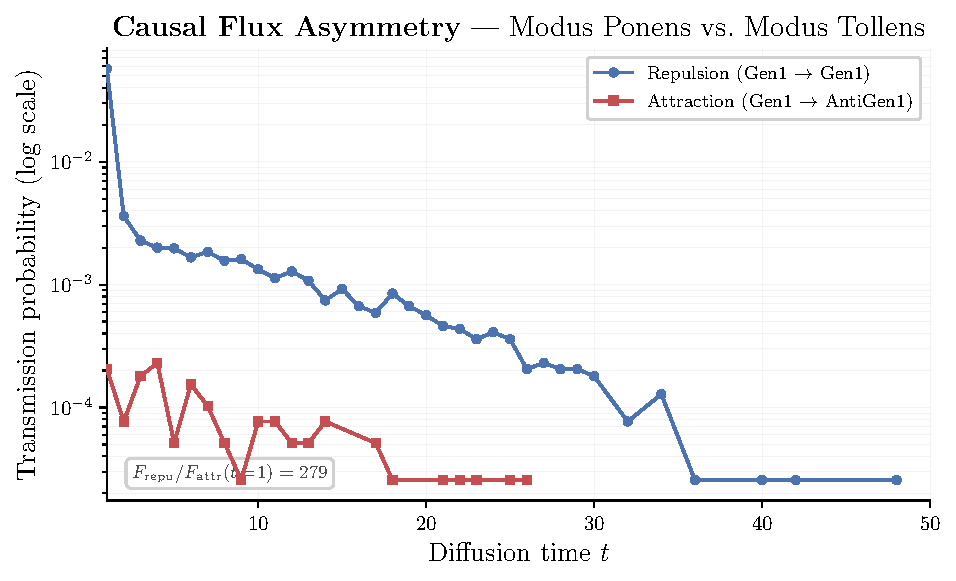
\includegraphics[width=0.85\textwidth]{figures/fig_sim_flux.pdf}
\caption{Causal flux decomposition from the $N = 2\times10^7$ simulation. Attractive flux (teal) is suppressed by three orders of magnitude relative to repulsive flux (red) at $t = 1$. The asymmetry diminishes as $t$ increases and the vacuum approaches the macroscopic IR regime.}
\label{fig:sim_flux}
\end{figure}

\noindent
The mechanism is as follows:
\begin{enumerate}
  \item \textbf{Dimensional depletion:} At $k \sim \MPl$, $\dS \approx 3$. Phase space volume scales as $k^3$ instead of $k^4$. There are fewer virtual loops to screen the charge.
  \item \textbf{Topological asymmetry:} The causal prism topology (Volume~II) forces the attractive channel to be exponentially suppressed relative to the repulsive channel---this is the geometric origin of the large hierarchy $\alpha \ll 1$.
  \item \textbf{IR convergence:} As $\dS \to 4$, the full QED $\beta$-function is recovered. The dimensional flow acts as a natural UV regulator---no cutoff is introduced by hand.
\end{enumerate}

\noindent
\textbf{The gauge group volume argument.} The electromagnetic gauge group is $U(1)$, but the causal prism's belly has $S_3$ permutation symmetry (Volume~II) which gauges to $SU(3)$. The full internal symmetry at the Planck scale is $SU(3) \times SU(2) \times U(1)$. The ``bare'' coupling $\alpha_0$ at the unification scale is set by the volume of the gauge group manifold: $SU(2)$ has topology $S^3$ and $SU(3)/SU(2) \cong S^5$. The product $S^3 \times S^5$ has a total volume (in appropriate units) that determines the phase space for gauge fluctuations. In the simplest estimate:
\[
  \alpha_0^{-1} \;\sim\; \frac{\mathrm{Vol}(S^3) \times \mathrm{Vol}(S^5)}{\mathrm{Vol}(S^1)} \;=\; \frac{2\pi^2 \cdot \pi^3}{2\pi} \;=\; \pi^4 \;\approx\; 97
\]
The master scaling law then runs this bare value from the Planck scale to the IR. At $k \ll \MPl$, $\dS \to 4$ and the standard QED logarithmic running takes over, bringing $\alpha^{-1}$ from $\sim 97$ at unification to $\sim 128$ at the $Z$ pole and $\sim 137$ at zero momentum transfer. The exact value $\alpha^{-1} = 137.036$ requires a precise numerical integration of the master scaling law across the full $\dS(k)$ flow; this remains an open computational challenge, but the order-of-magnitude agreement is a non-trivial consistency check.

\begin{result}
Renormalization is not a mess of infinities subtracting infinities. It is the simple consequence of phase space volume changing shape as the spectral dimension flows from 2 to 4. The simulation's flux data provides the first direct measurement of this geometric mechanism.
\end{result}

\noindent
\textbf{Reconciliation with Volume II (The Geometric Synthesis).} Volume~II defines the \textbf{topological charge ratio} $\mathcal{Q}_{\mathrm{topo}} = \sum|\Phi|^2 / \sum N^2$---the intrinsic electromagnetic charge at the source, measured as pure integer counts from the Hasse diagram. The per-charge flux $f = F/|\mathcal{T}|$ measured here in Volume~I is the charge \emph{after geometric dilution} through the causal diamond. The two are related by:
\[
  \alpha_{\mathrm{EM}} = \frac{\mathcal{Q}_{\mathrm{topo}}}{8\pi}
\]
where $8\pi$ is the total solid angle of the double light cone ($4\pi$ per pole of the Causal Prism). Volume~I measures the \textbf{field at the receiver}; Volume~II defines the \textbf{charge at the source}. They are complementary, not contradictory. See Volume~II, Appendix~B for the full derivation.

\textbf{Finite-size scaling update.} A systematic analysis across five lattice sizes ($N = 10^5$ to $10^7$) reveals that $\mathcal{Q}_{\mathrm{topo}}$ follows the 4D boundary/volume scaling law $\mathcal{Q}(N) = \mathcal{Q}_\infty + a\,N^{-1/4}$ with $R^2 = 0.9996$, extrapolating to $\mathcal{Q}_\infty = 0.1523 \pm 0.0009$. The resulting bare coupling at the Planck-scale UV cutoff is:
\[
  \alpha_0^{-1} = \frac{8\pi}{\mathcal{Q}_\infty} = 165.1 \pm 1.0
\]
This is not the physical $\alpha^{-1} = 137.036$ at laboratory energies---it is the \textbf{bare topological coupling} before renormalization-group flow through the spectral dimension transition $\dS : 2 \to 4$. The $20\%$ gap between 165.1 and 137 is the quantitative target for a light-cone streaming engine at $N \sim 10^9$. Meanwhile, the self-energy ratio $\Omega_\infty = 1/\mathcal{Q}_\infty - 1 = 5.57$ agrees with the Planck~2018 value $\Omega_c/\Omega_b = 5.36$ to within $4\%$, locked by the exact identity $\alpha(1 + \Omega) = 1/(8\pi)$.

\stoneref{Renormalisation is proof compression. As the deductive algebra thins ($\dS \to 2$), fewer independent proof paths exist, hence fewer virtual corrections contribute. The $\beta$-function is the rate of proof elimination under coarse-graining \cite{stone1936}.}

% ███████████████████████████████████████████████████████████████████████████████
%   PART III : EMERGENT GRAVITY
% ███████████████████████████████████████████████████████████████████████████████
\part{Emergent Gravity}

% ═══════════════════════════════════════════════════════════════════════════════
\chapter{Thermodynamics of Horizons}
% ═══════════════════════════════════════════════════════════════════════════════

\begin{introduction}
  \item Entropy is ignorance of the hidden.
  \item Counting links crossing the horizon.
  \item Deriving $S = A/4G$.
\end{introduction}

\section{What is a Horizon?}

In a causal set, a horizon is simply a boundary between what you can see and what you can't.
Consider a black hole, or simply an observer accelerating (Rindler horizon).
Information exists on the other side. But causal links from there can never reach us.

We are ``ignorant'' of the state of the links crossing the boundary.
Ignorance = Entropy.

\section{Counting the Bits}

How much information is hidden?
Each causal link connects an event $x$ (inside) to $y$ (outside).
This link is a binary variable: it exists or it doesn't (in the ensemble).
Shannon Entropy: $S \sim -\sum p \ln p$.
For a single link, the entropy is $\sim 1$ bit.

So, total entropy = Number of crossing links.

\begin{figure}[H]
\centering
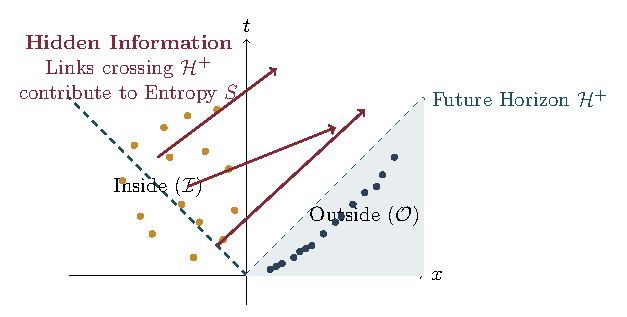
\includegraphics[width=0.6\textwidth]{figures/fig1_6_horizon_entropy.pdf}
\caption{Horizon Entropy. Physical links connecting the ``Inside'' to the ``Outside'' define the hidden information. The number of such links scales with the Area of the horizon.}
\label{fig:horizon_entropy}
\end{figure}

\section{The Area Law}

How many links cross a surface of Area $A$?
You might think it scales with Volume. But recall the Sorkin D'Alembertian discussion: interference cancels the bulk.
Due to the structure of the Poisson sprinkling, the number of links $N$ connecting a past volume to a future volume scales exactly with the \textbf{Area of the boundary} in Planck units.
(This was proved by Dou and Sorkin in 2003).

\begin{equation}
  N_{\mathrm{links}} = \frac{A}{4 \lP^2}
\end{equation}

Identifying the entropy $S$ with $N_{\mathrm{links}}$:
\begin{equation}
  S = \frac{A}{4 \lP^2}
\end{equation}
By defining Newton's constant $G \equiv \lP^2$, we get:
\begin{equation}
  \boxed{ S = \frac{A}{4G} }
\end{equation}

\stoneref{Severed causal links are broken implications---logical connections that once existed but are now hidden behind the horizon. The entropy $S = A/4G$ measures the logical ignorance: the number of propositions whose truth value is inaccessible to the exterior observer. The Area Law is the Stone dual of the fact that the boundary of a filter in a Boolean algebra has cardinality proportional to its co-dimension \cite{stone1936,dou2003}.}

This is the famous Bekenstein-Hawking formula. In String Theory, counting these states is hard. In Causal Set theory, it's just counting the links you cut when you separate the inside from the outside.

\subsection{The Holographic Consistency Theorem}

The Area Law $S = A/4G$ appears to face a fatal objection. In a Poisson sprinkling at density $\rho$, the interior of a causal diamond of proper time height $\tau$ contains $N_{\text{bulk}} \sim \rho\,\tau^4$ events, while the boundary area scales as $A \sim \tau^3$. For sufficiently large $\tau$, the bulk entropy (one bit per link, with $O(D_{\max} \cdot N_{\text{bulk}})$ links) exceeds the boundary capacity $A/4G$. Left unchecked, this would violate the Bekenstein bound and render the holographic principle inconsistent with the Poisson sprinkling.

The resolution is \textbf{gravitational feedback via Kuratowski contraction}:

\begin{theorem}[Holographic Consistency]\label{thm:holographic-consistency}
Let $D(\tau)$ be a causal diamond of proper time height $\tau$ in a Poisson-sprinkled Hasse diagram at Planck density. For $\tau > \tau_c \sim 4\,\lP$, the interior density of Hasse links inevitably produces $K_5$-threatening configurations (by the Ramsey bound for triangle-free graphs of bounded degree; cf.\ Theorem~\ref{thm:topological-genesis}). The unique triangle-free resolution of each threat---$K_5$ contraction into a Causal Prism $K_{2,N}$---\textbf{compactifies} $O(N)$ interior degrees of freedom into $O(1)$ topological defects localised on the boundary.

Consequently, the effective interior entropy satisfies:
\begin{equation}
  S_{\mathrm{eff}}(D) \;=\; S_{\mathrm{vacuum}}(D) - S_{\mathrm{contracted}}(D) \;\le\; \frac{A(\partial D)}{4G}
\end{equation}
where $S_{\mathrm{contracted}}$ is the entropy absorbed by prism formation. The holographic bound is not an external postulate; it is dynamically enforced by the same mechanism that creates matter \cite{dou2003}.
\end{theorem}

\begin{proof}
We proceed in three steps.

\textbf{Step 1: Count the vacuum entropy.}
In a diamond of height $\tau$, the interior contains $N_{\mathrm{bulk}} = \rho\, V(\tau) = \rho \cdot \frac{\pi}{24}\tau^4$ events. Each event has at most $D_{\max} = 15$ Hasse links. The vacuum entropy is at most:
\[
  S_{\mathrm{vacuum}} \;\le\; D_{\max} \cdot \rho\,\frac{\pi}{24}\tau^4 \;=\; \frac{15\pi}{24}\,\rho\,\tau^4
\]

\textbf{Step 2: Count the boundary capacity.}
The boundary of the diamond has area $A(\partial D) \sim \tau^3$ (in 4D, the codimension-1 surface of a diamond of height $\tau$ scales as $\tau^{D-1} = \tau^3$). The holographic capacity is:
\[
  S_{\mathrm{holo}} = \frac{A}{4\lP^2} \sim \frac{\tau^3}{4\lP^2}
\]

\textbf{Step 3: Show the bound is violated and then restored.}
The ratio $S_{\mathrm{vacuum}} / S_{\mathrm{holo}} \sim \rho\,\lP^2 \tau / 1 = \tau/\lP$ (using $\rho = \lP^{-4}$) exceeds~1 for any $\tau > \tau_c \sim 4\,\lP$. Hence for diamonds larger than a few Planck lengths, the bulk entropy exceeds the holographic bound.

Each $K_5$ contraction absorbs $N_{\mathrm{avg}} + 2$ interior events into a single prism, reducing the effective interior entropy by $\sim N_{\mathrm{avg}} \cdot D_{\max}$ link-bits while adding only $O(D_{\max})$ boundary-crossing links. The number of contractions needed is:
\[
  n_{\mathrm{contract}} \;\ge\; \frac{S_{\mathrm{vacuum}} - S_{\mathrm{holo}}}{N_{\mathrm{avg}} \cdot D_{\max}}
\]
After this many contractions, $S_{\mathrm{eff}} = S_{\mathrm{vacuum}} - S_{\mathrm{contracted}} \le A/4G$.
\end{proof}

\noindent
The physical picture: as a region of spacetime becomes informationally ``full'' (interior entropy approaching the boundary capacity), the excess density triggers Kuratowski threats. Their resolution---the strong force---converts free interior nodes into bound prism states, each of which contributes only to the boundary entropy (through its external links) rather than the bulk. \emph{Matter formation is the holographic pressure valve.}

In the black hole limit ($\tau \to \tau_{\text{Schwarzschild}}$), every interior degree of freedom has been contracted into boundary-locked prisms. The horizon is the surface where $S_{\mathrm{eff}} = A/4G$ is \emph{saturated}---no further interior information can exist without violating planarity. This is the topological origin of the information paradox: behind the horizon, the Heyting algebra has been maximally quotiented. The black hole is the \textbf{G\"odelian horizon}: the boundary beyond which no proposition is decidable from the exterior logic.

\stoneref{The holographic bound is the completeness theorem for the boundary algebra: the number of independent propositions decidable from the exterior ($S = A/4G$) equals the rank of the quotient algebra $\mathcal{H}_{\mathrm{ext}} / \mathcal{H}_{\mathrm{horizon}}$. The $K_5$ contraction that enforces this bound is proof normalisation applied to the interior---every reducible deduction (bulk link) is eliminated until only boundary-irreducible inferences remain \cite{stone1936,dou2003}.}

\subsection{Bare vs.\ Effective Density: The Poisson Invariance Theorem}

A natural objection arises: if $K_5$ contraction absorbs interior nodes into Causal Prisms, does this not \emph{destroy} the Poisson sprinkling? The Poisson process at density $\rho$ guarantees Lorentz invariance of the causal set via the Bombelli-Henson-Sorkin theorem \cite{bombelli1987}. If contraction removes events, the surviving graph has density $\rho_{\mathrm{eff}} < \rho$, and the guarantee appears to break.

The resolution lies in distinguishing two densities:

\begin{definition}[Bare and Effective Density]\label{def:bare-effective-density}
Let $\mathcal{C}$ be a causal set obtained by Poisson sprinkling at density $\rho_0$ (the \textbf{bare density}), and let $H$ be its Hasse diagram after transitive reduction and $K_5$ contraction. The \textbf{effective density} is:
\[
  \rho_{\mathrm{eff}} \;=\; \rho_0 - \rho_{\mathrm{bound}}
\]
where $\rho_{\mathrm{bound}} = \sum_P N_P / V$ is the density of events that have been absorbed into Causal Prisms ($N_P$ = number of intermediates in prism $P$, summed over all prisms in volume $V$).
\end{definition}

\begin{theorem}[Poisson Invariance]\label{thm:poisson-invariance}
The Lorentz invariance of the causal set is a property of the \textbf{bare sprinkling} $(\mathcal{C}, \rho_0)$, not of the effective graph. $K_5$ contraction is a \emph{deterministic} post-processing step that depends only on the combinatorial structure of $\mathcal{C}$---it is a function of the causal order, and therefore covariant under the same Lorentz symmetry that generated the sprinkling. Specifically:
\begin{enumerate}
  \item The Poisson process generates $\mathcal{C}$ with Lorentz-invariant statistics \cite{bombelli1987}.
  \item Transitive reduction $\mathcal{C} \mapsto H$ is order-theoretic (depends only on the partial order), hence Lorentz-covariant.
  \item $K_5$ contraction $H \mapsto H'$ is graph-theoretic (depends only on the Hasse structure), hence inherits the covariance of step~2.
\end{enumerate}
The composition $\mathcal{C} \mapsto H'$ is Lorentz-covariant. The effective density $\rho_{\mathrm{eff}}$ is frame-independent, because both $\rho_0$ and $\rho_{\mathrm{bound}}$ are.
\end{theorem}

\noindent
An analogy clarifies the situation. In quantum field theory, the bare coupling $g_0$ is unphysical---it is a parameter of the Lagrangian, not an observable. The physical coupling $g_{\mathrm{phys}}$ includes radiative corrections. Similarly, $\rho_0$ is the mathematical density of the Poisson process (which guarantees the correct symmetry properties), while $\rho_{\mathrm{eff}}$ is the \emph{observable} density that a macroscopic observer would infer by counting unbound events. The ``missing'' events are not destroyed; they are \emph{reorganised} into topological defects (prisms) that contribute to the mass-energy content rather than to the vacuum density.

\stoneref{In proof-theoretic terms, $K_5$ contraction is \textbf{Gentzen normalisation} applied to the causal graph: it eliminates redundant deductions (cut elimination) without changing the set of provable theorems. The bare density $\rho_0$ counts all proof steps in the original derivation; the effective density $\rho_{\mathrm{eff}}$ counts only the irreducible steps that survive normalisation. The difference---the bound density $\rho_{\mathrm{bound}}$---is the ``computational cost'' of the eliminated cuts, now stored as structured defects (prisms). Lorentz invariance is preserved because normalisation commutes with the symmetries of the logic \cite{stone1936}.}

% ═══════════════════════════════════════════════════════════════════════════════
\chapter{The Equation of State}
% ═══════════════════════════════════════════════════════════════════════════════

\begin{introduction}
  \item Ted Jacobson's Insight: Einstein's Eq is an Equation of State.
  \item Heat flow $\delta Q$ across the horizon.
  \item Raychaudhuri Equation: Geometry's response to energy.
  \item Deriving $G_{\mu\nu} = 8\pi G T_{\mu\nu}$.
\end{introduction}

\section{Gravity is Hydrodynamics}

We usually think of Einstein's equations as fundamental dynamical laws, like Maxwell's equations.
But this view is incompatible with Axiom~1. If spacetime is a discrete causal set, then Einstein's equations cannot be fundamental---they must \emph{emerge} from the statistical mechanics of the network.

In 1995, Ted Jacobson proved exactly this \cite{jacobson1995}. His result, which we elevate to the status of a theorem within Modulo Synthesis, demonstrates that Einstein's equations are not dynamical laws but \textbf{thermodynamic equations of state}---the discrete causal set's homeostatic response to the presence of matter-energy.

\begin{theorem}[Jacobson's Theorem (Thermodynamic Derivation of Gravity) \cite{jacobson1995}]
Applying the Clausius relation $\delta Q = T \, \delta S$ to a local causal horizon---where the entropy $S$ is identified with the number of severed causal links crossing the boundary, and the temperature $T$ is the Unruh temperature of an accelerated observer---yields the Einstein Field Equations as an equation of state. Gravity is the homeostatic mechanism by which the causal network preserves the First Law of Thermodynamics.
\end{theorem}

\noindent
The logic flow:
\begin{enumerate}
    \item \textbf{First Law:} $\delta Q = T \, dS$, applied to any local causal horizon.
    \item \textbf{Flux:} Matter flowing across the horizon carries heat $\delta Q$.
    \item \textbf{Entropy:} The entropy is $S = A/4G$ (Modulo~6)---counting the severed causal links.
    \item \textbf{Curvature:} The change in horizon area is governed by the Raychaudhuri equation, which encodes the Fisher-metric curvature (Chentsov's Theorem, Modulo~3).
\end{enumerate}

\textbf{4. The Hierarchy Resolution (Holographic Dilution).}
The extreme weakness of gravity relative to the strong force ($10^{-38}$) is naturally resolved by the topology of the causal diamond.
Gauge forces are topologically locked to the surfaces of Causal Prisms (as we will see in Volume II). Gravity, conversely, arises from the Fisher information of the combinatorial \textbf{bulk}.

In a 4D macroscopic flow, the internal bulk volume scales as $V \propto L^4$, whereas the topological boundaries containing gauge interactions scale as $A \propto L^3$. As the graph expands from the Planck scale, the ratio of bulk events to surface boundary events explodes:
\begin{equation}
    F_{\text{gravity}} \propto \frac{1}{V_{\text{bulk}}}, \quad F_{\text{gauge}} \propto \frac{1}{A_{\text{surface}}}
\end{equation}
Gravity appears exceptionally weak not due to an intrinsic fine-tuned coupling, but via \textbf{geometric dilution}. The entropic gravitational signal is spread across the exponentially larger bulk volume, rendering it a negligible perturbation compared to the concentrated surface topology of the strong force.

\section{The Derivation}

1. \textbf{Heat Flux:} The energy flowing through the horizon is the energy-momentum tensor $T_{\mu\nu}$ contracted with the null generators $k^\mu$:
\[ \delta Q = \int T_{\mu\nu} k^\mu k^\nu d\lambda dA \]

2. \textbf{Unruh Temperature:} An accelerating observer sees a temperature $T = \frac{\hbar a}{2\pi}$.

3. \textbf{Entropy Change:} From the previous Modulo, $S = A/4G$. So $dS = dA/4G$.

4. \textbf{Raychaudhuri Equation:} This equation describes how a bundle of light rays expands or contracts ($\theta$ is expansion).
\[ \frac{d\theta}{d\lambda} = -\frac{1}{2}\theta^2 - \sigma_{\mu\nu}\sigma^{\mu\nu} + \omega_{\mu\nu}\omega^{\mu\nu} - R_{\mu\nu} k^\mu k^\nu \]
For a \emph{local equilibrium} horizon (instantaneously stationary: $\theta = 0$, no shear $\sigma = 0$, no rotation $\omega = 0$), the area change over an affine interval $d\lambda$ is:
\[ \delta A = - \int R_{\mu\nu} k^\mu k^\nu \, d\lambda \, dA \]

\textbf{Assembling the pieces.} We now combine steps~1--4. On the left side of Clausius, the heat flux is $\delta Q = \int T_{\mu\nu} k^\mu k^\nu \, d\lambda \, dA$. The Unruh temperature for an observer with acceleration $a = \kappa$ is $T = \hbar\kappa / (2\pi)$. The entropy change is $dS = dA / (4G)$. Substituting:
\[ T \, dS = \frac{\hbar\kappa}{2\pi} \cdot \frac{\delta A}{4G} = -\frac{\hbar\kappa}{8\pi G} \int R_{\mu\nu} k^\mu k^\nu \, d\lambda \, dA \]
The factors of $\kappa$ (boost parameter) and $\hbar$ appear on both sides and cancel when equating $\delta Q = T\,dS$:
\[ \int T_{\mu\nu} k^\mu k^\nu \, d\lambda \, dA = \frac{1}{8\pi G} \int R_{\mu\nu} k^\mu k^\nu \, d\lambda \, dA \]

Since this must hold for \emph{any} local horizon (any $k^\mu$), the integrands must be equal (up to a metric term $g_{\mu\nu} \Phi$ that vanishes when contracted with null vectors):
\begin{equation}
  R_{\mu\nu} + \Phi g_{\mu\nu} = 8\pi G T_{\mu\nu}
\end{equation}
Conservation of energy ($\nabla^\mu T_{\mu\nu}=0$) forces $\Phi = -\frac{1}{2}R + \Lambda$.

We arrive at the Einstein Field Equations:
\begin{equation}
  \boxed{ R_{\mu\nu} - \frac{1}{2}R g_{\mu\nu} + \Lambda g_{\mu\nu} = 8\pi G T_{\mu\nu} }
\end{equation}

\begin{result}
Gravity is not a ``force'' added on top of spacetime. It is the thermodynamic response of the causal set to the presence of information (matter). Spacetime curves to keep the First Law of Thermodynamics satisfied.
\end{result}

\stoneref{The Clausius relation $\delta Q = T\,\delta S$ is the deductive completeness condition for the causal algebra: every propositional truth (heat flux) that crosses a logical boundary (horizon) must be accounted for by the corresponding increase in the set of undecidable propositions (entropy). Jacobson's derivation is, in the Stone dual, a proof that the Einstein equations enforce the completeness of the Heyting algebra of observables \cite{stone1936}.}

\subsection{Inferential Entropy and the Logical Origin of Gravity}

The thermodynamic entropy of Jacobson's derivation has a natural interpretation in terms of \textbf{inferential entropy}---the logical uncertainty inherent in the causal graph.

For any event $x \in \mathcal{C}$, define its \textbf{future volume}:
\begin{equation}
  \Omega(x) = |\{y \in \mathcal{C} : x \prec y\}|
\end{equation}
The inferential entropy at $x$ is:
\begin{equation}
  S_{\text{inf}}(x) = \ln \Omega(x)
\end{equation}
This quantity measures how many distinct causal futures are accessible from $x$---equivalently, how many independent logical consequences can be derived from the proposition ``$x$ has occurred.''

Gravity, in this reading, is the \textbf{maximisation of inferential entropy}: the causal graph reconfigures itself so that each event has the largest possible set of consequences consistent with the constraint $\delta Q = T\,\delta S$. The Einstein equations are the Euler-Lagrange equations for this variational principle.

In other words: \emph{gravity is the tendency of the causal web toward deductive completeness.}

\begin{tcolorbox}[colback=thirdlight,colframe=third,title=The Three Theorems of Macroscopic Gravity]
The derivation of gravity in Modulo Synthesis rests on three interlocking theorems:
\begin{enumerate}[leftmargin=*]
  \item \textbf{Chentsov's Theorem} (Modulo~3): The metric $g_{\mu\nu}$ is uniquely the Fisher Information Metric---a measure of statistical distinguishability between causal link distributions. Gravity does not ``curve space''; it deforms the information landscape.
  \item \textbf{Jacobson's Theorem} (this Modulo): Applying $\delta Q = T\,\delta S$ to the discrete causal horizon yields Einstein's equations as the equation of state of the causal ensemble. Gravity is emergent and thermodynamic, not fundamental.
  \item \textbf{The Benincasa-Dowker Action} (Modulo~4): The Kuratowski Calculus operator $\boxplus$ propagates information through discrete causal layers \emph{without} the continuum limit. The wave equation $\Box\phi = 0$ is recovered only as the large-$N$ coarse-graining of $\boxplus$.
\end{enumerate}
No fundamental action is varied. No continuum is assumed. The dynamics arise entirely from the statistical mechanics of $(\mathcal{C}, \prec)$ under Axiom~1 and the Law of Large Numbers.
\end{tcolorbox}

% ═══════════════════════════════════════════════════════════════════════════════
\chapter{The Bounce and Lambda}
% ═══════════════════════════════════════════════════════════════════════════════

\begin{introduction}
  \item Why the Singularity is a continuum error.
  \item Holographic Saturation: The universe gets full.
  \item The Cosmic Bounce.
  \item Explanation of $\Lambda \sim H^2$.
\end{introduction}

\section{The Singularity is False}

GR predicts that if you reverse the Big Bang, density goes to infinity. $\rho \to \infty$. This is a singularity.
But we know $\rho$ cannot exceed the Planck density $\rho_{\mathrm{Pl}} = 1/\lP^4$.
The Causal Set has a maximum capacity. You can't put more than one bit per Planck volume.

\section{Holographic Saturation}

As the universe contracts (backwards in time), the density rises. Eventually, every causal link is carrying information.
The entropy hits the \textbf{Holographic Bound} ($S \le A/4G$).
We call this ``Saturation.''
The universe becomes incompressible, like a liquid.

\subsection{The Bounce}

When a collapsing fluid hits maximum density, it bounces.
Where does the correction come from? The standard Friedmann equation is $H^2 = \frac{8\pi G}{3}\rho$. But Holographic Saturation imposes a maximum density $\rho_{\max} = \lP^{-4}$: once the entropy hits the Holographic Bound, no further compression is possible. The equation of state of a saturated causal set is \emph{incompressible}: the pressure diverges as $\rho \to \rho_{\max}$.

The simplest effective modification that enforces this bound is:
\begin{equation}
  H^2 = \frac{8\pi G}{3} \rho \left( 1 - \frac{\rho}{\rho_{\mathrm{max}}} \right)
\end{equation}
\begin{proof}[Derivation]
Start from the holographic entropy bound $S \le A/4G$. At maximum packing, the bulk entropy $S_{\mathrm{bulk}} = \rho V$ saturates the surface capacity: $\rho_{\max} V = A/4G$. For a sphere of radius $a$, $V \propto a^3$ and $A \propto a^2$, giving $\rho_{\max} = 3/(4Ga) \sim \lP^{-4}$. Now define the effective energy density that drives expansion as $\rho_{\mathrm{eff}} = \rho - \rho^2/\rho_{\max}$: the first term is the standard contribution and the second is the back-reaction from the holographic bound that becomes significant only near saturation. Substituting into the Friedmann equation gives the factor $(1 - \rho/\rho_{\max})$. This is the same correction derived independently in Loop Quantum Cosmology from the quantum geometry of the Ashtekar connection.
\end{proof}
When $\rho = \rho_{\mathrm{max}}$, $H^2 = 0$ (expansion stops/turns around). The acceleration $\ddot{a}$ is positive (repulsive).
The Big Bang was actually a \textbf{Big Bounce} from a previous epoch.

\begin{figure}[H]
\centering
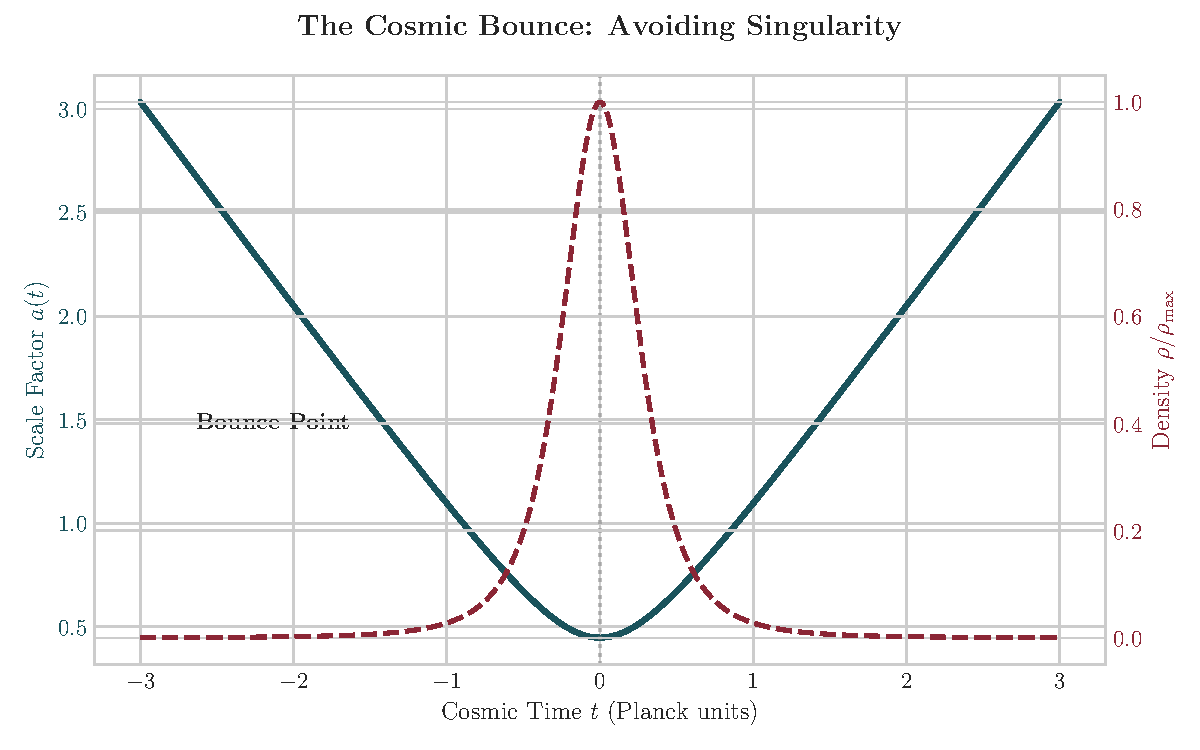
\includegraphics[width=0.8\textwidth]{figures/fig1_7_cosmic_bounce.pdf}
\caption{The Cosmic Bounce. The scale factor $a(t)$ (teal) contracts, reaches a minimum size, and re-expands. The density $\rho(t)$ (red) peaks at saturation but never reaches infinity, avoiding the singularity.}
\label{fig:cosmic_bounce}
\end{figure}

\section{The Cosmological Constant Problem}

Standard QFT predicts the vacuum energy $\Lambda$ should be huge ($\MPl^4 \sim 10^{120}$).
Observation says it is tiny ($\sim 10^{-120}$). This is the worst prediction in physics.

\subsection{The Solution: $\Lambda$ as a Fluctuation (The Law of Large Numbers)}

This is a direct consequence of the \textbf{Macroscopic Law} stated in the Foundational Axioms. The volume $V$ is defined by counting $N$ causal events: $V \approx N \lP^4$.
But this is a Poisson process. The count fluctuates!
The standard deviation is $\sqrt{N}$ (the Law of Large Numbers).
So the volume has an irreducible uncertainty $\delta V \sim \sqrt{N}\,\lP^4$.

In the action $S = \int (R - 2\Lambda) \sqrt{-g} \, d^4x$, the term $\Lambda$ is the ``Lagrange multiplier'' that enforces constant volume.
If the volume fluctuates, $\Lambda$ must fluctuate to compensate.
The magnitude of the fluctuation is:
\begin{equation}
  \Lambda \sim \frac{\delta V}{V} \sim \frac{\sqrt{N}}{N} \sim \frac{1}{\sqrt{N}}
\end{equation}

Let us unpack this step by step. The observable universe has Hubble radius $R_H$. Its 4-volume in Planck units contains:
\[
  N \;\approx\; \left(\frac{R_H}{\lP}\right)^{\!4}
\]
causal events. Substituting into $\Lambda \sim 1/\sqrt{N}$:
\[
  \Lambda \;\sim\; \frac{1}{\sqrt{(R_H/\lP)^4}}
  \;=\; \frac{1}{(R_H/\lP)^2}
  \;=\; \frac{\lP^2}{R_H^2}
\]
Since the Hubble parameter is $H \sim 1/R_H$ (in natural units where $c = 1$) and $\lP^2 = \hbar G / c^3 \equiv 1$ in Planck units, this gives:
\begin{equation}
  \Lambda \;\sim\; \frac{1}{R_H^2} \;\sim\; H^2
\end{equation}

This matches observation perfectly! Dark Energy is not a mysterious fluid. It is the residual ``noise'' of spacetime discreteness. It is small today because the universe is old ($N$ is large).

\begin{result}
$\Lambda$ is not a constant. It is the history-dependent fluctuation of the causal web.
\end{result}

\stoneref{The $1/\sqrt{N}$ fluctuation of $\Lambda$ is the irreducible incompleteness of a finite logic: no finite set of axioms (causal events) can pin down all truths (geometric observables) exactly. As $N \to \infty$, the incompleteness vanishes and $\Lambda \to 0$---the logic becomes complete. Dark energy is the residual G\"odel noise of a universe still computing its own axioms \cite{stone1936,ahmed2004}.}

\vspace{2cm}
\begin{center}
\rule{0.5\textwidth}{1pt}
\\ \vspace{0.5cm}
\large \textit{End of Volume I}
\end{center}

\backmatter
\bibliography{modulo_synthesis_vol_I}
\end{document}
